\documentclass[11pt]{book}
\usepackage[usenames,dvips,pdftex]{color}
\usepackage[pdftex]{color,graphicx}
\usepackage{hyperref}
\usepackage{array}
\usepackage{tabularx}
\usepackage{overpic, epic}
\usepackage{float}
\usepackage{textcomp}
\hypersetup{colorlinks=true, filecolor=black, linkcolor=black, urlcolor=blue, citecolor=black}


\graphicspath{{./images/}}

\begin{document}
\title{PR2 user manual}
\author{Willow Garage}
\newcommand{\TODO}[1]{\textcolor{red}{TODO: #1}}
\maketitle
\newpage
\tableofcontents
\newpage
\chapter {Introduction}
This manual is intended to give you enough information to successfully install, use, and develop code on your PR2 robot.  The software on the PR2 is provided by software based on ROS.  The recommended source of information for learning about ROS and the higher-level software available for the PR2 is http://ros.org

If you want to get started running the PR2 as quickly as possible, please start with Chapter 2 on safety (seriously - the PR2 is a big machine and can cause serious injuries or death), and then you can skip to chapter 5 to learn how to start up and run the PR2.

\section{Before you start}
\paragraph{Space} To use PR2 you will need to have enough room for it to drive around and move it's arms.  The PR2 is designed to move through ADA-compliant spaces (Americans with Disabilities Act), so corridors should be at least 36" wide, doorways should be at least 32", and the ground should be flat and level.  You will need enough space for the PR2 to move around and perform tasks.
\paragraph{Safe Environment} The space where the PR2 operates should be free of hazards.  Specifically, stairways or other fall hazards can pose an extreme danger and the PR2 should not be operated near any type of dropoff.  You should also avoid hazardous objects, such as knives, sources of fire, hazardous chemicals, or furniture that could be knocked over.  See chapter 2 for more details on making sure your environment is safe.
\paragraph{Electrical} The PR2 recharges using a standard 120V American power outlet.  The robot can draw 15A of current when plugged in, so we strongly recommend recharging the PR2 only on outlets with no other devices on the circuit breaker.
\paragraph{Development tools}
You will need at least one laptop or desktop computer to use to connect to the robot.  The PR2 ships with a base-station computer, which is a desktop, but you will need to provide a screen, mouse, and keyboard.  A laptop with wireless access is ideal.
\paragraph{Linux} We highly recommend familiarity with the Linux command-line.  The PR2 computers both run Ubuntu, and since they don't have attached displays, all tasks on them have to be performed by logging in remotely (e.g. via ssh).
\paragraph{ROS} Since all the PR2 software is based on ROS, running through the beginning tutorials available at ROS.org will help you understand the structure of the software on the robot and will give you tools to understand the software that's running and the data that is moving around in the system.
\paragraph{PR2 Safety} Be sure to familiarize yourself with the contents of the following chapter on safety before using the PR2.


\chapter{Safety}

Safety is a key goal at Willow Garage.  It is important, it is challenging, and it is a continual process shared by the designer, user, and administrator of a robot.  In the following we provide an overview of the issues, describe some safety-related design features, enumerate a set of basic usage guidelines to support safety, and finally detail the explicit safety program.

\section{Overview}

Safety is a vitally important concern whenever you are around a PR2. It is a heavy piece of equipment with many moving parts. It travels though the environment and can carry and manipulate a wide variety of objects. Its movements and actions are not completely predictable. It can cause significant damage if it falls on or runs over someone. There are several ways it can pinch, grab, and twist fingers or other parts of the body. It can wield dangerous implements and knock heavy things over. You must always be cautious and attentive when you are around a PR2.

Safety is neither absolute criterion nor a one-time event.  Instead it is an appreciation that risks are inherent to any robotic endeavor and they must be minimized as well as weighed against benefits.  It is a goal for which the entire community must continually strive.

We emphasize safety to avoid harm to any person, animal, or equipment.  We also recognize that robots in general will not gain wide acceptance or fulfill their potential unless the community can adequately manage safety.

Managing safety is challenge when dealing with any complex engineering system.  In the case of the PR2, consider also the open, extensible, programmable, experimental nature of the platform.  The PR2's capabilities and behaviors change over time, with user interactions, and with re-programming.

With this in mind, Willow Garage has chosen a three-fold approach.  First, we have designed the PR2 to minimize potential risks and maximize inherent safety, cognizant of its uncertain uses.  Second, we communicate to all users about how to minimize risk. And third, we have implemented an explicit safety program to ensure that the community continues to identify potential hazards, seek design mitigations, and communicate effective usage guidelines.

\section{Design Features}

We have designed both hardware and software to minimize risks, while retaining the power of an open platform.  These aspects of the design are often described as inherent safety features.  For example, PR2's arms are back-drivable.  That means when an arm encounters an object, be it a table or a person, the interaction will drive the motors back and bring the arm to a stop.  The PR2 arms can't "punch through" an object the way traditional industrial robots can.

We have further designed the PR2 arms with relatively small motors with respect to their payload.  This is possible due to a spring counterbalance offsetting the gravity forces acting on the arms.  That is, the arms do not need to hold their own weight against gravity.  And so the motors need only be strong enough to hold the payload.  The arms simply can't push very hard.

In software, we have incorporated low level checking to limit the current in a motor, to limit the velocity of a motor, and to limit the range through which a motor should travel.  We obviously discourage users and developers from changing these configurations.  High level applications also avoid obstacles in navigation and movement using the various on-board sensors.

These design choices also help make PR2 robust.  However, a robot with the PR2's capabilities can never be absolutely safe. Your safety as well as the safety of others critically depends on your constant attention. You must be aware of the potential dangers, anticipate possible problems, and plan to prevent their occurrence.

\section{General Usage Guidelines}

While many guidelines for the safe use of a robot stem from common sense, we enumerate a basic set here.  We stress the importance of following these guidelines but re-emphasize that these guidelines alone do not guarantee safety but reduce risk.
\begin{itemize}
\item Every organization that uses a PR2 must appoint a Safety Officer.
\begin{itemize}
\item The Safety Officer's contact information should be known by everyone in the organization who uses the PR2 (including designers, developers, programmers, and end-users).
\item Further details of the Safety Officer's roles and responsibilities are described in section 2.4.
\end{itemize}
\item Before operating or working with the PR2 you must do the following:
\begin{itemize}
\item view the safety video
\item read this User Manual, particularly Chapter 2 on Safety
\item read and understand the latest list of potential hazards
\item know how to contact your organization's Safety Officer
\end{itemize}
\item Supervise children, visitors, and anyone who has not followed the previous guideline.  In particular, make sure they
\begin{itemize}
\item do not come within range of the PR2 when active
\item are aware the robot could move unexpectedly and is potentially dangerous
\item are not alone with the PR2
\item do not operate the PR2
\end{itemize}
\item Maintain a safe environment.  Safety is not only an issue of how you operate the robot, but also the environment.
\begin{itemize}
\item Make sure the robot has adequate and level space for any expected or unexpected operation
\item Make sure the the environment is free of objects that could pose a risk if knocked, hit, or otherwise affected by the PR2
\item Make sure no animals are the near the robot.
\end{itemize}
\item The PR2 is designed to operate in an laboratory environment
\begin{itemize}
\item It should not be operated outdoors
\item It should not come in contact with liquids
\item It should not be operated within 7 meters of the top of a stairway
\end{itemize}
\item Anticipate potential problems and hazards.  Always imagine what might happen if the robot malfunctions or behaves in a way different from the desired action.  Be vigilant.
\item The operator should always have immediate access to the run/stop and stop the robot at the first sign of a problem.
\item Use common sense when operating the robot.
\begin{itemize}
\item Do not allow the robot to grab or hit any person
\item Do not allow the robot to drive into contact with or over any body part.
\item Do not allow the robot to interact with any sharp or dangerous items
\end{itemize}
\item Pay attention to warning labels on the robot.
\item Do not remove the covers of a PR2 without prior and appropriate instruction by Willow Garage. There are high voltages and a variety of pinching and other mechanical dangers in the interior of the robot.
\item Do not modify or remove any part of the software safety features.
\end{itemize}

\section{Safety Program}

Safety is a continual process, and in particular should include

\begin{itemize}
\item an awareness of risks
\item a critical examination to expose risks, assess risks, discover mitigations, and evaluate trade-offs
\item any deliberate actions needed to minimize and mitigate current and future risks.
\end{itemize}

To facilitate this process and communication within the community, Willow Garage has implemented a safety program.

\subsection{Willow Garage Safety Board}

The Willow Garage Safety Board identifies hazards related to Willow Garage products and ensures that appropriate actions are taken to mitigate those hazards. The Board maintains a database to keep track of the hazards and mitigation actions. To identify additional hazards for the database, the Board commissions Hazard Brainstorming Meetings and reviews incident reports from the field. To initiate actions that reduce the severity and/or likelihood of specific hazards, the Board commissions Hazard Response Projects. To ensure that appropriate actions remain in force, the Board commissions Hazard Response Audits. The Board works with Safety Officers in external organizations to improve safety across all users of Willow Garage products.
The core Safety Board includes senior members of the Willow Garage management. Additional employees serve for term appointments. Members of the Board spend at least one day a month on safety related work.
\subsection{Hazard Database}

The Hazard Database includes three types of entity: Hazards, Incidents, and Responses.
Hazards describe things the system might do that can cause damage, for example, running into something or falling down stairs. Each Hazard includes an estimate of its severity and likelihood of occurrence. Based on these estimates, the Hazard is assigned a priority for action.
Incidents describe specific examples of Hazards, either things that have actually occurred or hypothetical occurrences. Each Incident is associated in the database with the Hazard(s) that it exemplifies.
Responses describe actions that reduce the severity and/or likelihood of a hazard. These can involve changes to the design or documentation of the hardware and software, additional warnings to the community, or changes to the safety training and video.

The information in the Hazard Database is summarized in several reports that document the current understanding of potential hazards and the associated mitigating actions. Chief among these is the Prioritized Hazard Report, which lists the Hazards in the database in order of their priority.

\subsection{Safety Officers}

Each organization that uses Willow Garage products will appoint a Safety Officer who is responsible for all aspects of safety in the use of those products. The Safety Officer will:
\begin{itemize}
\item remain informed of all known safety hazards and mitigations,
\item ensure that all known mitigations are implemented in their organization,
\item ensure that everyone involved with the products receives safety training,
\item report any safety incidents to Willow Garage in a timely fashion, and
\item work with the Willow Garage Safety Board to improve safety.
\end{itemize}

\chapter{Safety and the PR2}
Point out which parts of the code are considered part of the hardware safety systems (e.g. joint current limits), 
and make it clear that changing them can cause problems.

Talk about guidelines for safe operation (e.g. is it OK in a normal lab environment?)

\chapter{PR2 hardware}

\section{What's in the box}
THe PR2 ships in 3 packages:

\begin{tabular}{| l | l |}
\hline      
  Main robot crate & Large wooden crate which contains the PR2 itself \\ \hline
  Accessory crate & Crate which contains accessory kit, tool kit, and robot base-station \\ \hline
  Calibration target & Large checkerboard for accurate calibration of stereo cameras \\ \hline
\end{tabular}

\subsection{PR2}
\subsection{Accessory kit}
\subsubsection{Wireless Joystick}
The PR2 ships with a bluetooth joystick for teleoperating the robot. The bluetooth joystick is a 
\href{http://www.sonystyle.com/webapp/wcs/stores/servlet/ProductDisplay?catalogId=10551&storeId=10151&langId=-1&productId=8198552921665411965#additionalImage1%22}{Sony DUALSHOCK®3} (Figure~\ref{fig:ps3joy}) 
wireless controller. It can be charged using any standard USB A to mini-B USB cable. For more information, see the 
\href{http://www.ros.org/wiki/ps3joy}{ps3joy} package at \href{http://www.ros.org}{ros.org}.

\begin{figure}[h]
\centering
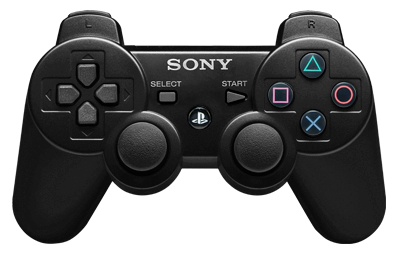
\includegraphics[scale=0.5]{ps3joy.png}
\caption{The PR2 bluetooth joystick.}
\label{fig:ps3joy}
\end{figure}

\subsubsection{Wireless run-stop}
\label{wirelessrunstop}
The PR2 comes with an \href{http://www.omnexcontrols.com/products/portable/t50.html}{OMNEX T50} 
wireless run-stop transmitter. When stopped or out of range, the wireless run-stop transmitter will halt the motors 
and put the power system in standby mode. 

\begin{figure}[h]
\centering
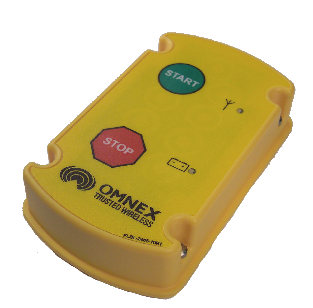
\includegraphics[width=150px]{run_stop.png}
\caption{The PR2 wireless run-stop.}
\label{fig:runstop}
\end{figure}

To start the run-stop, press the green start button (Figure~\ref{fig:runstop}); if this works properly, you will see a 
light flashing on the run-stop. While transmitting, the run-stop has a range of approximately 800 ft. The run-stop is 
powered by four AA batteries; the battery light will flash when the battery charge is low, which is an indication that 
you should change the batteries.

\TODO{Create and fill out subsection for every component of accessory kit}

\subsection{Toolkit}
\TODO{Include image of open toolkit, with callout labels to all tools by proper name}
\TODO{TBD: The robot toolkit is not yet fully defined}

\subsection{Calibration target}
The calibration target which ships with the robot will be is a checkerboard 1" thick and approximately 3 feet on a side.  This is the recommended calibration target to use for calibrating the intrinsics of the stereo cameras on the robot.  The robot ships with stereo cameras already calibrated, but you may need to re-calibrate occasionally as vibration and thermal effects change the parameters over time.

\subsection{Base-station computer}
\TODO{Include picture of base-station here}
The base-station computer ships without a monitor, keyboard, or mouse.  See section ??? for more information on how to configure your base-station.

\section{Mechanism}
PR2 is a 32-dof mobile manipulator with a mobile base, two arms, and a variety of sensors on a pan-tilt head.

\subsection{Robot Anatomy}

Kinematically speaking, the PR2 can be broken down into {\bf links} by individual degrees of freedoms.  Each {\bf link} consist of one
rigid body component that can be represented by a single collision model and a single lumped inertial property.
All links are interconnected together by {\bf joint} constraints in the form of revolute, prismatic or fixed {\bf joints}.
In this literature, a revolute joint without limits is also called a continuous joint.
In general, the entire PR2 mechanism is represented by a tree where each node is a {\bf link}
  and the edges connecting individual nodes are {\bf joints}.
In the tree representation of the PR2, each node (link) can be connected (via joints) to only one parent node but can have arbitrarily many child nodes.

A link without collision or inertial components is referred to as a {\bf frame}. Frames are always rigidly attached to parent links via fixed joints and cannot have children links.
A frame serves an important function of facilitating transform record keeping through our \href{http://www.ros.org/wiki/tf}{Transform and Frames Library (TF)}
  for propagating information such as reference coordinates of an optical image, origin of range sensor generated point cloud data or the reference pose for the grasp point of a gripper.

A CAD approximated kinematic and inertial description of the PR2 can be found
  in the \href{http://www.ros.org/wiki/pr2\_description}{pr2\_description} package.
This package uses a robot specific Extensible Markup Language (XML) and Document Object Model (DOM) representation
  called \href{http://www.ros.org/wiki/urdf}{Uniform Robot Description Format(URDF)} created here at Willow Garage.

Rather than diving into all 32 DOF's of the PR2 in detail right away, the next section examines the robot by its major components:  head, torso, arms, base and casters.
This overall breakdown of the PR2 robot is depicted in Figure~\ref{fig:pr2_basic_breakdown}.

\subsubsection{Head}
The PR2 head consists of two links: {\bf head\_pan\_link} and {\bf head\_tilt\_link}.  The {\bf head\_tilt\_link} is attached via a revolute joint called {\bf head\_tilt\_joint} to the {\bf head\_pan\_link}.
The {\bf head\_pan\_link} is attached to the PR2 torso ({\bf torso\_lift\_link}) by another revolute joint called the {\bf head\_pan\_joint}.

The individual head sensors are detailed separately in the section~\ref{subsec:pr2_sensors}

\subsubsection{Arms}
The PR2 arms can be further subdivided into shoulder, upper arm, forearm and gripper.  Each components is separately described in detail below:
\begin{itemize}
\item Shoulers
  \begin{itemize}
  \item {\bf l\_shoulder\_pan\_link} {\bf r\_shoulder\_pan\_link}
  \item {\bf l\_shoulder\_lift\_link} {\bf r\_shoulder\_lift\_link}
  \item {\bf l\_upper\_arm\_roll\_link} {\bf r\_upper\_arm\_roll\_link}
  \end{itemize}
\item Upper Arms
  \begin{itemize}
  \item {\bf l\_upper\_arm\_link} {\bf r\_upper\_arm\_link}
  \item {\bf l\_elbow\_flex\_link} {\bf r\_elbow\_flex\_link}
  \item {\bf l\_forearm\_roll\_link} {\bf r\_forearm\_roll\_link}
  \end{itemize}
\item Forearms
  \begin{itemize}
  \item {\bf l\_forearm\_link} {\bf r\_forearm\_link}
  \item {\bf l\_wrist\_flex\_link} {\bf r\_wrist\_flex\_link}
  \item {\bf l\_wrist\_roll\_link} {\bf r\_wrist\_roll\_link}
  \end{itemize}
\item Grippers
  \begin{itemize}
  \item {\bf l\_gripper\_palm\_link} {\bf r\_gripper\_palm\_link}
  \item {\bf l\_gripper\_l\_finger\_link} {\bf l\_gripper\_r\_finger\_link}
        {\bf r\_gripper\_l\_finger\_link} {\bf r\_gripper\_r\_finger\_link}
  \item {\bf l\_gripper\_l\_finger\_tip\_link} {\bf l\_gripper\_r\_finger\_tip\_link}
        {\bf r\_gripper\_l\_finger\_tip\_link} {\bf r\_gripper\_r\_finger\_tip\_link}
  \end{itemize}
\end{itemize}


\subsubsection{Torso}
The PR2 {\bf torso\_lift\_link} refers to the torso part of the PR2 that moves up and down with the elevator actuator.

\subsubsection{Base}
The PR2 {\bf base\_link} is the lower part of the PR2 body, housing the PR2 computers and is also rigidly attached to the base Hokuyo laser scanner.

\subsubsection{Casters}
The PR2 has 4 caster units.  Each caster contains one actuated steering degree of freedom and two individually actuated wheels.

\subsubsection{Home Pose}
In order to describe the PR2 robot pose and joint positions in a consistent manner, a {\bf home pose} of the robot has been defined.  The {\bf home pose} is described in detail in section~\ref{sec:pr2_coordinate_system}.

\subsubsection{Sensors}
\label{subsec:pr2_sensors}
Details of the PR2 sensors are described here.
The PR2 contains the following sensors:
\begin{itemize}
\item Image Sensors
  \begin{itemize}
  \item Dual Stereo Cameras
    \begin{itemize}
    \item Narrow Stereo Camera Pair
    \item Wide Stereo Camera Pair
    \end{itemize}
  \item Prosilica Camera
  \item Forearm Cameras
  \end{itemize}
\item Range Sensors
  \begin{itemize}
  \item Tilting Hokuyo Laser Scanner
  \item Base Hokuyo Laser Scanner
  \end{itemize}
\item Accelerometers
  \begin{itemize}
  \item IMU
  \item Gripper Palm Mounted Accelerometers
  \end{itemize}
\end{itemize}


\subsubsection{PR2 Coordinate System}
\label{sec:pr2_coordinate_system}
The reference {\bf home pose} of the PR2 robot is defined as the robot pose with all the joint angles at zero,
with the PR2 robot facing the positive x-direction, positive z-axis pointing upwards and positive y-axis pointing to the {\it robot-left} (see Figure~\ref{fig:pr2_home_pose}).

\begin{figure}[!h]
\centering
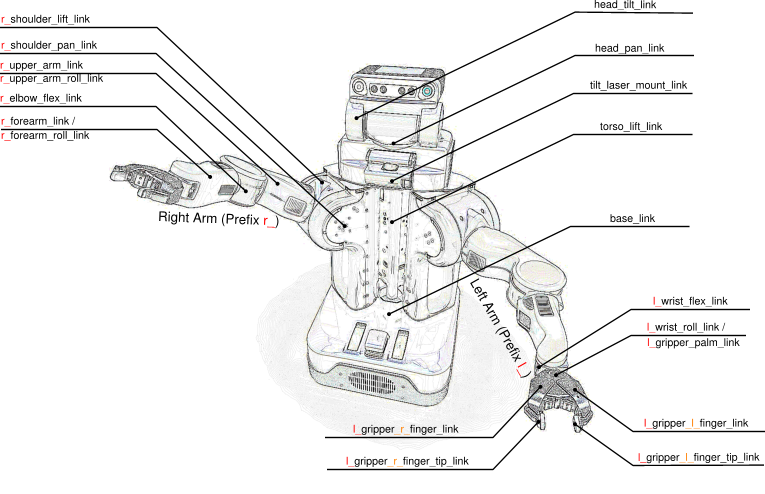
\includegraphics[scale=0.3]{urdf_links.png}
\caption{The PR2 URDF Link Naming Scheme.}
\label{fig:urdf_link_names}
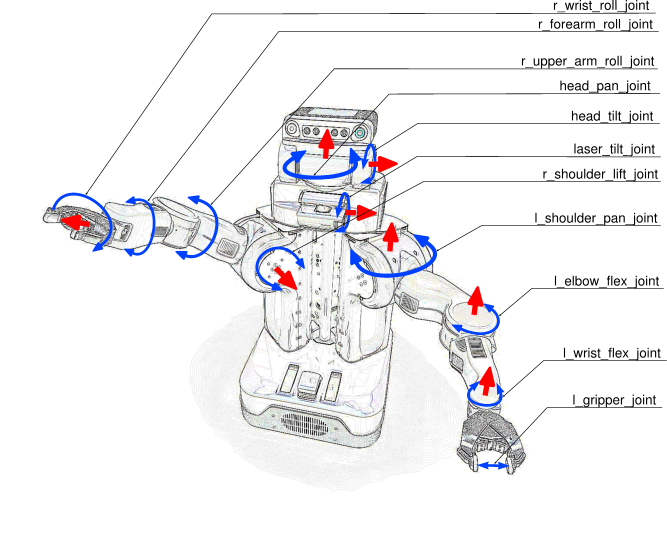
\includegraphics[scale=0.3]{urdf_joints.png}
\caption{The PR2 URDF Joints Naming Scheme.}
\label{fig:urdf_joints}
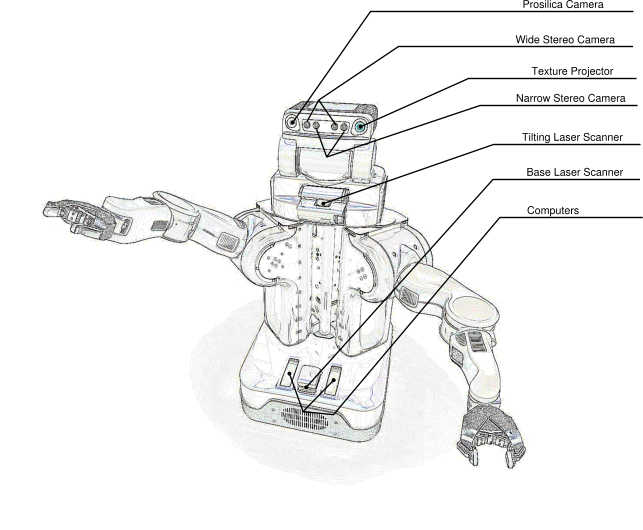
\includegraphics[scale=0.3]{urdf_sensors.png}
\caption{The PR2 Sensors.}
\label{fig:urdf_sensor}
\end{figure}

\subsection{Drivetrains}
The PR2 drivetrains have been designed to be low inertia and
backdrivable with minimal backlash. There are three types of
drivetrains on the PR2, gear drives, belt drives, and lead screw
drives.  

\subsubsection{Belt Drives}
The most common drivetrain on the PR2 is the belt drive.  

The typical link drivetrain is a DC motor with attached encoder.  It
runs through a planetary gearbox then is attached to a belt
drive. These drivetrains are fully backdriveable and have low
backlash.

%\TODO{Belt drive Diagram}
\paragraph{Standard Belt Drives}
The following motors use belt drives as described above: Caster Wheel,
Caster Turret, Head Tilt, Shoulder Pan, Shoulder Lift, and the Upper
Arm Roll.
\paragraph{Semi-Standard Belt Drives}
The Upper Arm Flex is standard except that there is an additional 90
degree bevel gear pair on this joint between the gearbox and the belt
drive.  The Laser Tilt is standard except that there is no gearbox,
there is a flex coupler in it's place.  And the encoder is on the
mechanism side of the flex coupler.  The Head Pan is standard except
that the gearbox is replaced by gears, with the encoder on the
mechanism side of the gears.



\subsubsection{Gear Drives}
The wrist, head pan and forearm roll use gear drives.  

\paragraph{Wrist}
The wrist utilized a differential drive between two motors.  If they
are turned in the same direction the wrist rolls, if they are turned
oposite the wrist flexes.  The differential bevel gears are attached
after a standard encoder, motor, gearhead assembly.

\TODO {wrist diagram}

\paragraph{Forearm roll}
The forearm roll has a traditional encoder, motor, gearbox assembly
with a pinion gear attached to the output shaft.  The pinion gear
directly drives a nylon gear built into the forearm body.

\subsubsection{Lead Screw Drives}
There are two drive trains which use lead screws as their primary
method of movement, the torso lift and gripper.  

\paragraph{Torso Lift}
The torso lift is driven by a vertical lead screw.  The motor is
augmented by a gas spring vertically such that the motor only needs to
lift a portion of the weight of the torso.  The torso is also mounted
such that the lift mechanism cannot pull downward.

\paragraph{Gripper}
The gripper is a pair of 4 bar linkages which are coupled through a
gearing on one of the piviots.  The mechanism is actuated using a lead
screw between the two fourbar linkages. Between the actuator and the
gearing the movement of the grippers is limited to a single degree of
freedom.

The gripper is backdriveable when off, however challenging.
Backdriving the gripper when torque is applied is very hard, but
possible.

\paragraph{Arm Counter Balance}
Although not an actuated drivetrain the arm counter balance is one of
the more complicated mechanisms on the PR2. Inside of the shoulder
turret there are two springs.  These springs are attached to belts
which run over cams and provide a uniform downward force.

In the upper arm there is a four-bar linkage which transmits the
torque through to the elbow flex joint.  As the arm moves through its
configuration space the linkage changes the amount of leverage with
which the counterbalance is pulling which compensates for the
different configurations.

\subsubsection{Drivetrain Limitations}
The drivetrains are high fidelity however there are still limitations.
Below are the most observable limitations.

%\paragraph{Fault Conditions}
%\paragraph{Observed failures during testing}
%\begin{itemize}
%\item Belt broken \TODO {document counterbalance failure??}
%\item Stripped belt teeth
%\item Loose set screw
%\end{itemize}
%\paragraph{Running Errors}
%There has been no measured hysteresis or backlash in the drivetrains
%except in the two forms below.  \TODO{verify with vijay}

\paragraph{Belt Stretch}
On all the belt driven joints.  The belts do stretch when under load.
The stretching is small but measureable.

\paragraph{Encoder Discritization}
As the arm is moving slowly the discrete nature of the encoders can
become evident.  It usually manifests itself as a jitter in the
velocity.  It can be filtered out to some extent, but not too much for
it will cause lag.



Discuss the drive-train approach, how/why things work, what types of errors we expect to see and don't expect to see

\subsection{Motion control}


\begin{figure}[h]
\centering
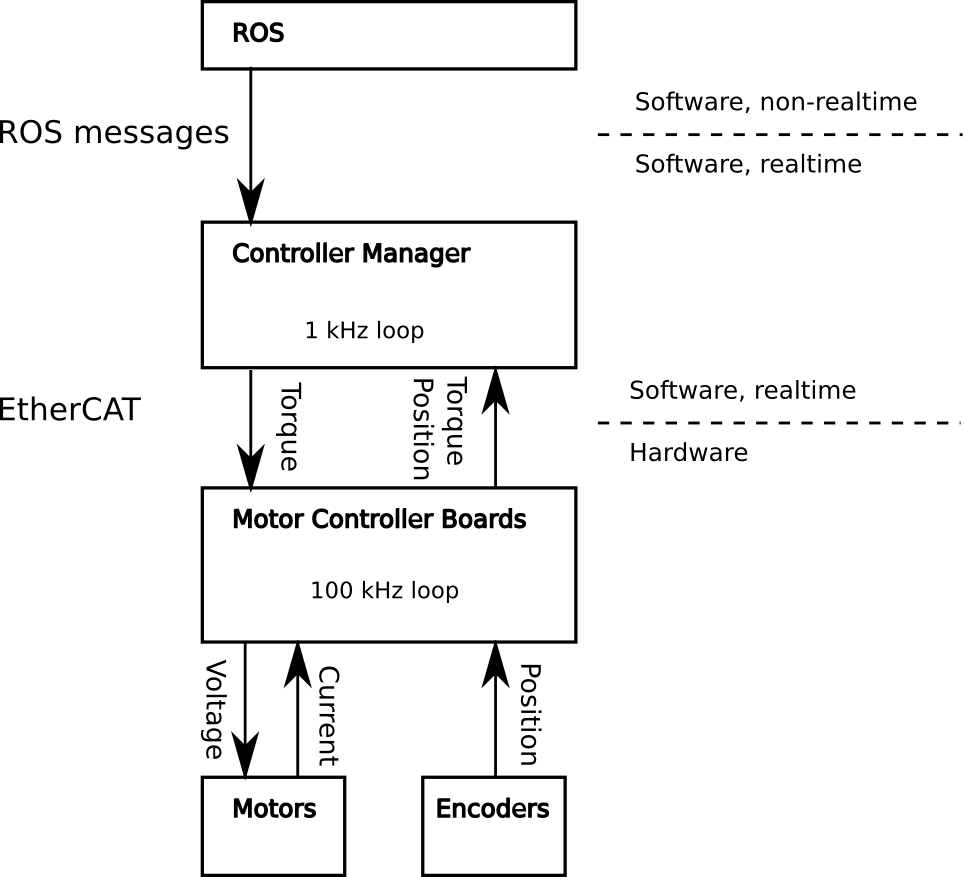
\includegraphics[width=290px]{images/mechanism_control.png}
\caption{Motion control layout.}
\label{fig:motion_control}
\end{figure}


\subsubsection{Motor controller boards}
Each motor/encoder on the PR2 has its dedicated \emph{Motor Controller
  Board} (MCB). The MCB detects and counts transitions in the encoder
signal, measures the current the motor is using, and commands the
voltage going to the motor. Each MCB runs a PI-control loop to control
the motor current to a desired value, by commanding the motor
voltage. This control loop is executed at 100~kHz on an FPGA.  A
shared etherCAT link allows all MCB's in the PR2 to communicate with
the main computers.

\subsubsection{Controller manager}
The \emph{Controller Manager} (CM) is the lowest level software
component that directly talks to the MCB's. The CM runs in a hard
realtime process and is guaranteed to be executed at 1~kHz. This means
the CM sends desired motor torques to the MCB's every milisecond, and
receives measured motor torques and positions in the same milisecond.

The CM has a dynamic plugin loading mechanism that allows controller
algorithms to get inserted and executed inside the 1~kHz realtime
loop.


\subsection{Mechanical specs}

Before undertaking any new or risky operations with your PR2, please consult these mechanical specifications. Do not operate the PR2 outside of these specifications. If you have any questions about your PR2's specifications, please contact Willow Garage Support.

\subsubsection{Environmental specs}

The PR2 is an indoor, household robot. Operating outside this type of environment could cause damage to the PR2, or injury or death to operators.

\paragraph{Water}

The PR2 has not been tested for any type of contact with water or any other liquid. Under no circumstances should the PR2 come in contact with water from rain, mist, ground water (puddles) or liquid handling. Water contact can cause damage to the electrical circuitry and the mechanism.

\paragraph{Temperature and Humidity}

Temperature testing of the PR2 has allowed the unit to run between 15 and 35C. Temperatures outside of this range can cause malfunctions in the PR2 power system and instruments. The PR2 has been tested in high humidity, but under no circumstances should condensation be allowed to form on the vehicle.

\paragraph{Drive Surface}

The drive surface of the PR2 must be capable of supporting the entire weight of the PR2, about 450 pounds (220 kgs). If the surface is too soft, the PR2 can get stuck and fail to drive. A commercial carpet or tile is recommended. 

\paragraph{Incline Surface}

The PR2 is ready for ADA compatible ramps, which specifies a 1/12 slope. Ramps that are steeper than 1/12 slope are unsafe and may be a tip over hazard.

\paragraph{Other Environmental Specs}

\begin{itemize}
\item UV exposure should be minimized. UV radiation can damage the PR2's skin
\item Dust and dirt can clog air filters
\end{itemize}

\subsubsection{Forces and torques}

Joint position, velocity, and force limits are implemented in the PR2's URDF file, in the ``/etc/ros/urdf/robot.xml" file on your PR2. These joint limits control the range of travel of the mechanism, the allowable velocity to prevent overtravel. These limits are enforced by pr2\_controller\_manager, and are designed to prevent poorly designed controllers from damaging the PR2 and harming operators. 



The limits below are from the PR2 URDF file. If a velocity or torque limit is not specified, no value is enforced by pr2\_controller\_manager.

\begin{tabular}{l*{2}{c}}
Joint  & Velocity (rad/s or m/s) & Torque (Nm or N) \\
\hline \hline
$\ast$\_caster\_rotation\_joint        & -     & -  \\
$\ast$\_caster\_wheel\_$\ast$\_joint   & -     & -  \\
torso\_lift\_joint                     & 0.013 & 10000 \\
laser\_tilt\_joint                     & 10.00 & 0.65  \\
head\_pan\_joint                       & 6.00  & 2.65  \\
head\_tilt\_joint                      & 5.00  & 15.00 \\
$\ast$\_shoulder\_pan\_joint           & 2.10  & 30.00 \\
$\ast$\_shoulder\_lift\_joint          & 2.10  & 30.00 \\
$\ast$\_upper\_arm\_roll\_joint        & 3.27  & 30.00 \\
$\ast$\_elbow\_flex\_joint             & 3.30  & 30.00 \\
$\ast$\_forearm\_roll\_joint           & 3.60  & 30.00 \\
$\ast$\_wrist\_flex\_joint             & 3.10  & 10.00 \\
$\ast$\_wrist\_roll\_joint             & 3.60  & 10.00 \\
$\ast$\_gripper\_joint                 & 0.20  & 1000  \\
\end{tabular}

The PR2 motor controller boards (MCB's) will not allow a current command greater than the maximum continuous current specified for the joint's actuator. This means that maximum joint effort may be lower than the maximum effort specified above. Below are the actuators for each joint (Maxon part number), and their maximum allowable commanded current. 

\begin{tabular}{ll*{2}{c}}
Joint  & Motor & Power (W) & Max Current \\
\hline \hline
$\ast$\_caster\_rotation\_joint       & 236672 & 20  & 0.655 \\
$\ast$\_caster\_wheel\_$\ast$\_joint  & 236672 & 20  & 0.655 \\
torso\_lift\_joint                    & 148877 & 150 & 3.12  \\
laser\_tilt\_joint                    & 310009 & 60  & 1.72  \\
head\_pan\_joint                      & 310009 & 60  & 1.72  \\
head\_tilt\_joint                     & 310009 & 60  & 1.72  \\
$\ast$\_shoulder\_pan\_joint          & 148877 & 150 & 3.12  \\
$\ast$\_shoulder\_lift\_joint         & 148877 & 150 & 3.12  \\
$\ast$\_upper\_arm\_roll\_joint       & 148877 & 150 & 3.12  \\
$\ast$\_elbow\_flex\_joint            & 148877 & 150 & 3.12  \\
$\ast$\_forearm\_roll\_joint          & 310009 & 60  & 1.72  \\
$\ast$\_wrist\_flex\_joint            & 310009 & 60  & 1.72  \\
$\ast$\_wrist\_roll\_joint            & 310009 & 60  & 1.72  \\
$\ast$\_gripper\_joint                & 222057 & 11  & 0.204 \\
\end{tabular}

More information about each actuator may be found in Maxon datasheets.

\subsubsection{Joint Limits and Types}

The position limits for the PR2 are specified below. These ``hard limits" are the maximum travel for the mechanism. 

\begin{tabular}{ll*{2}{c}}
Joint  & Type  & Limit (+) & Limit (-) \\
\hline \hline
$\ast$\_caster\_rotation\_joint        & continuous & -            & - \\
$\ast$\_caster\_wheel\_$\ast$\_joint   & continuous & -            & - \\
torso\_lift\_joint                     & prismatic  & 310 mm       & 0 mm \\
laser\_tilt\_joint                     & revolute   & 85$^\circ$   & 45$^\circ$ \\
head\_pan\_joint                       & revolute   & 168$^\circ$  & 168$^\circ$  \\
head\_tilt\_joint                      & revolute   & 60$^\circ$   & 30$^\circ$  \\
r\_shoulder\_pan\_joint                 & revolute   & 40$^\circ$   & 130$^\circ$  \\
l\_shoulder\_pan\_joint                 & revolute   & 130$^\circ$  & -40$^\circ$  \\
$\ast$\_shoulder\_lift\_joint          & revolute   & 80$^\circ$   & 30$^\circ$  \\
r\_upper\_arm\_roll\_joint              & revolute   & 44$^\circ$   & -224$^\circ$  \\
l\_upper\_arm\_roll\_joint              & revolute   & 224$^\circ$  & -44$^\circ$  \\
$\ast$\_elbow\_flex\_joint             & revolute   & 133$^\circ$  & 0$^\circ$  \\
$\ast$\_forearm\_roll\_joint           & continuous & -            & - \\
$\ast$\_wrist\_flex\_joint             & revolute   & 130$^\circ$  & 0$^\circ$  \\
$\ast$\_wrist\_roll\_joint             & continuous & -            & - \\
$\ast$\_gripper\_joint                 & prismatic  & 86 mm        & 0 mm \\
\end{tabular}

\subsubsection{Modifying Joint Limits}

On the PR2, ``soft limits" stop the joints from reaching the full range of motion to prevent damage to the mechanism. These soft limits, similar to a virual spring, are specified in the robot's URDF file. For an explanation of their implementation, see http://www.ros.org/wiki/pr2\_controller\_manager/safety\_limits.

The soft limits have been carefully implemented and validated by Willow Garage. Under no circumstances should they be changed without prior written authorization by Willow Garage Safety. Unauthorized and unvalidated modification of these limits could cause mechanism damage and injury or death to PR2 operators. 

Changing maximum allowable effort or maximum actuator current could cause serious damage to the PR2 and injury or death to operators. 

\section{Sensors}
The PR2 has a variety of sensors spread out over it's body:\\\\
\begin{overpic}[scale=0.45]{sensors.png}
\put(46.9,50.9){\href{http://www.ros.org/wiki/prosilica_camera}{
\includegraphics[scale=0.45]{sensors_prosilica.png}}}
\put(49,51){\href{http://www.ros.org/wiki/wge100_camera}{
\includegraphics[scale=0.45]{sensor_camera.png}}}
\put(55.3,50.9){\href{http://www.ros.org/wiki/}{
\includegraphics[scale=0.45]{sensors_projector.png}}}
\put(47.6,43.7){\href{http://www.ros.org/wiki/hokuyo_node}{
\includegraphics[scale=0.45]{sensors_tilt_laser.png}}}
\put(43.05,19.9){\href{http://www.ros.org/wiki/hokuyo_node}{
\includegraphics[scale=0.45]{sensors_base_laser.png}}}
\put(61.8,23.6){\href{http://www.ros.org/wiki/wge100_camera}{
\includegraphics[scale=0.45]{sensors_r_forearm.png}}}
\put(26.4,30.9){\href{http://www.ros.org/wiki/wge100_camera}{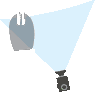
\includegraphics[scale=0.45]{sensors_l_forearm.png}}}
\end{overpic}

\subsection{Base Laser}
The base laser of the PR2 is \href{http://www.hokuyo-aut.jp/02sensor/07scanner/utm_30lx.html}{Hokuyo Top-URG (UTM-30LX)} 
scanning range finder that is located on PR2's base. This laser has a 30 m and 270$^\circ$ scanning range. For more information, 
see the \href{http://www.ros.org/wiki/hokuyo_node}{hokuyo\_node} package at \href{http://www.ros.org}{ros.org}.

\subsection{Tilting Laser}
\label{tilting laser}
In addition to the base laser, the PR2 has a \href{http://www.hokuyo-aut.jp/02sensor/07scanner/utm_30lx.html}{Hokuyo Top-URG (UTM-30LX)}
mounted on a tilting platform that is located just below the pan-tilt head. The tilting platform can sweep the scanning 
laser through 135$^\circ$ ($+90^\circ$ and $-45^\circ$ from level) and can be controlled using the
default laser\_tilt\_controller. For more information, see the \href{http://www.ros.org/wiki/hokuyo_node}{hokuyo\_node} 
and \href{http://www.ros.org/wiki/pr2_default_controllers}{pr2\_default\_controllers} packages at \href{http://www.ros.org}{ros.org}.

\subsection{Head Cameras}
The PR2 pan-tilt head has three cameras and a textured light projector:
\begin{description}
\label{stereo camera}
\item[Wide Stereo Camera]
The wide stereo camera of the PR2 is part of the dual stereo pair and is a 100Mb color ethernet camera. The wide stereo 
uses the \href{http://www.aptina.com/products/image_sensors/mt9v032c12stc/#overview}{Aptina MT9V032C12STC} imager chip
and has a maximum resolution of 752 x 480 pixels at 15 fps. The camera has a field of view (FOV) of approximately 
$90^\circ$ and a 2.5mm F2.5 \href{http://www.mars-cam.com/lenses/ccd_cmos/Technology%20Report(V-4402.5-2.5-HR).pdf}{Marshall V-4402.5-2.5-HR} 
lens. For more information, see the \href{http://www.ros.org/wiki/wge100_camera}{TODO} package
at \href{http://www.ros.org}{ros.org}.

\item[Narrow Stereo Camera]
The narrow stereo camera of the PR2 is part of the dual stereo pair and is a 100Mb monchrome ethernet camera. 
The narrow stereo uses the \href{http://www.aptina.com/products/image_sensors/mt9v032c12stm/#overview}{Aptina MT9V032C12STM} 
imager chip and has a max resolution of 752 x 480 pixels at 15 fps. The camera has a FOV of approximately $55^\circ$ and 
a 5.6mm F2.0  \href{http://www.mars-cam.com/lenses/ccd_cmos/Technology%20Report(V-4405.6-2.0-HR).pdf}{Marshall V-4405.6-2.0-HR}
lens. For more information, see the \href{http://www.ros.org/wiki/wge100_camera}{TODO} package
at \href{http://www.ros.org}{ros.org}.

\item[Gigabit Ethernet Camera]
\label{ethernet camera}
The PR2 has a gigabit ethernet camera located to the left of the dual stereo pair on the pan-tilt head. 
The gigabit ethernet camera is a \href{http://www.prosilica.com/products/gc2450.html}{Prosilica GC2450C},  
which uses the Sony ICX-625AQ imager chip and has a maximum resolution of 2448 x 2050 pixels at 15 fps. 
Additionally, the gigabit ethernet camera has a 8mm F1.4-F16 \href{http://www.kowascope.com/frontend/proddetail.asp?pn=LM8JC&co=10000348}{Kowa LM8JC} 
lens. For more information, see the \href{http://www.ros.org/wiki/prosilica_camera}{prosilica\_camera} 
package at \href{http://www.ros.org}{ros.org}.

\item[Textured Light Projector]
\label{texture projector}
The PR2 has a textured light projector located to the (robot's) left of the dual stereo pair on the pan-tilt head. 
The projector has a FOV of approximately $55^\circ$ and a 5.6mm F2.0 \href{http://www.kowascope.com/frontend/proddetail.asp?pn=LM12JC&co=10000348}{Kowa LM12JC} 
lens.  For more information, see the \href{http://www.ros.org/wiki/TODO}{TODO} package at \href{http://www.ros.org}{ros.org}.

\end{description}

\subsection{Forearm cameras}
Each forearm of the PR2 is equipped with a 12V 100Mb color ethernet camera. The forearm camera uses the 
\href{http://www.aptina.com/products/image_sensors/mt9v032c12stc/#overview}{Aptina MT9V032C12STC}  imager chip
and has a maximum resolution of 752 x 480 pixels at 15 fps. Additionally, the forearm camera has a 2.5mm F2.0 lens.  
For more information, see the \href{http://www.ros.org/wiki/wge100_camera}{wge100\_camera} package
at \href{http://www.ros.org}{ros.org}.

\subsection{Gripper Sensors}
\begin{description}

\item[Accelerometer]
The gripper of the PR2 is equipped with a \href{http://www.bosch-sensortec.com/content/language1/html/3474.htm}{Bosch BMA150} 
digital triaxal accelerometer. The measurement range ($\pm$2g, $\pm$4g, or $\pm$8g) and bandwidth (25Hz - 1500Hz) 
of the accelerometer can be selected in software. For more information, see the \href{http://www.ros.org/wiki/wge100_camera}{TODO} 
package at \href{http://www.ros.org}{ros.org}.

\item[Fingertip Pressure Sensors]
The default fingertips of the PR2 are sturdy aluminum blocks with non-slip 
rubber covers, for added friction and compliance in grasping.  However, the 
aluminum tips can be swapped out for an (included) set of RoboTouch tactile 
sensing pads made by Pressure Profile Systems, each with 22 tactile sensing 
elements: 15 in a 5x3 array on the front surface, 2 on top, 2 on each side, 
and 1 in back, near the top.  Each tactile element has a pressure range of 
0-30 psi (0-205 kPa) and sensitivity of 0.1 psi (0.7 kPa).  The sensors 
connect to the robot via an SPI ribbon cable and two screws, and have a 
maximum scan rate of 35 Hz.

The tactile sensors are highly fragile when not protected by the rubber 
covering, and so care should be taken not to damage the rubber covering when 
the tactile sensors are being used on the robot.  For more information, 
see the \href{http://www.ros.org/wiki/fingertip\_pressure}{fingertip\_pressure} package at \href{http://ros.org}{ros.org}.

\item[Calibration LED]

\end{description}

\subsection{Inertial measurement unit}
The PR2 has an inertial measurement unit (IMU) located next to the tilting laser. The IMU is a 
\href{http://www.microstrain.com/3dm-gx2.aspx}{MicroStrain Inertial-Link 3DM-GX2} which has an 
accelerometer range of $\pm$5g and a gyro range of $300^\circ/s$. For more information, see 
the \href{http://www.ros.org/wiki/microstrain_3dmgx2_imu}{microstrain\_3dmgx2\_imu} package 
at \href{http://www.ros.org}{ros.org}.

\subsection{Speaker}
The PR2 has one \href{http://www.logitech.com/index.cfm/speakers_audio/home_pc_speakers/devices/199&cl=us,en}{Logitech V20 notebook speaker} 
that is located under the pan-tilt head next to the tilting laser. For more information, 
see the \href{http://www.ros.org/wiki/sound_play}{sound\_play} package at \href{http://www.ros.org}{ros.org}.

\section{Power system}
\subsection{Overview}
The PR2 has a Lithium-ion (Li-ion) battery system that is charged off of 120V wall current. The batteries power the computers, motors, and sensors on the robot.  Power distribution is controlled by the \emph{Power Board}, which communicates over Ethernet.
\subsection{Power Busses}
The robot has four internal power busses:
\begin{description}
\item[120v] The robot has a 3-prong IEC320 plug in the back of the base, which is connected through a circuit breaker to the inputs of the four AC-DC converters that are used to charge the battery packs.  The system is designed to draw less than 15A, a standard 15A or 20A outlet will suffice. The load is capable at times of approaching the 15A limit, you should make sure there are no other devices which draw significant power on the same circuit (e.g., computers or heaters).
\underline{Ideally, add image of back panel once we have the PR2 betas done w/ Ryan's stickers on that panel.}
\item[Motor Power Bus] The motors get power through 3 descrete circuit breakers on the power board. 
These create three independent motor power busses: left arm, right arm, and base/head.
The motor power bus can be in one of three states.  
\emph{Enabled}, provides a direct connection to the unregulated battery power. The voltage will ranges from 52V when the batteries are fully discharged up to 72V when connected to wall power.  
\emph{Standby}, the power board provides a low-power 18V supply that is used for communication and maintaing encoder position counts.  
\emph{Disabled}, total shut-down of the circuit (e.g., in the event of a major power-system problem or manually disabled through the control panel).
\item[12V system bus]
12V power for sensors supplied by the power board. This is also the recommended source of power for user supplied accessories.
\item[12V computer power]
12V power for the computers supplied by the power board.
\end{description}
\subsection{Batteries}
The battery system has four battery bays comprised of four \href{http://www.oceanserver-store.com/18.html}{Ocean Server BA95HC-FL}
14.4V Li-ion batteries, a \href{http://www.v-infinity.com/adtemplate_child.asp?c=710918&p=903285&catky=764537&subcatky1=46887&subcatky2=320934}{V-INFINITY VF-S320-18A-CF}
18V AC-DC Power Supply, and a \href{http://www.oceanserver-store.com/xpmibamamo.html}{Ocean Server XP-04SRW} four-channel high 
current battery controller. This provides the PR2 with approximately two hours of countinous operation after a full recharge. 
For more information, see the \href{http://www.ros.org/wiki/ocean\_server}{ocean\_server} package at \href{http://www.ros.org}{ros.org}.

\subsection{Power board}
The power board is central to the PR2's power system. This is where the power from the batteries passes through to the rest of the system. The power board monitors total power drawn from the batteries by measuring the voltage and current at the power board input.

The battery power is used to provide regulated twelve volts to the computers and the system bus through DC converters. Three unregulated circuits are also provided with a unique electronic circuit breaker functionality. All outputs are ultimately controlled by the processor located on this board.


Here is an image of the power board, with e-stop receiver, removed from a robot.

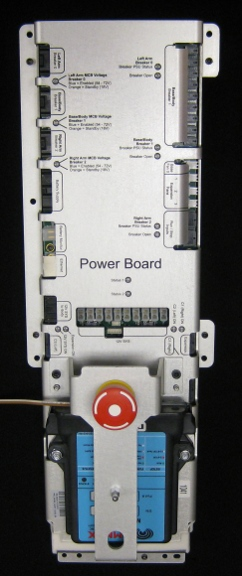
\includegraphics[scale=0.4]{pb_cropped1.jpg}


The power board contains an ARM processor with an ethernet interface. The processor is responsible for performing a self test at power-on, monitoring the state of all busses, providing information about the electrical system and responding to commands. The power board is the first thing to turn on and can not be turned off without switching off the DC circuit to the whole robot.

Besides supplying power the power board also interfaces with the emergency stop radio receiver and the emergency stop button. The emergency stop system is designed to reduce the power on the motor bus to a level where only the board communications and their encoder positions are maintained. The red button and radio system are described as providing a physical run/stop control over the motors in the robot. This description is used because this mechanism is implemented in hardware and can not be altered by software. 

Please note that the run/stop system only reduces power to the motor power bus and nothing else. If there is an electrical problem or power needs to be shutdown for service, the red circuit breaker on the rear lower panel is the only way to totally shut off the power board.

The power board contains many LEDs used to indicate status. I will show their locations and briefly describe their meanings.

The LEDs in green indicate the 3 regulated 12V outputs are enabled and functional.
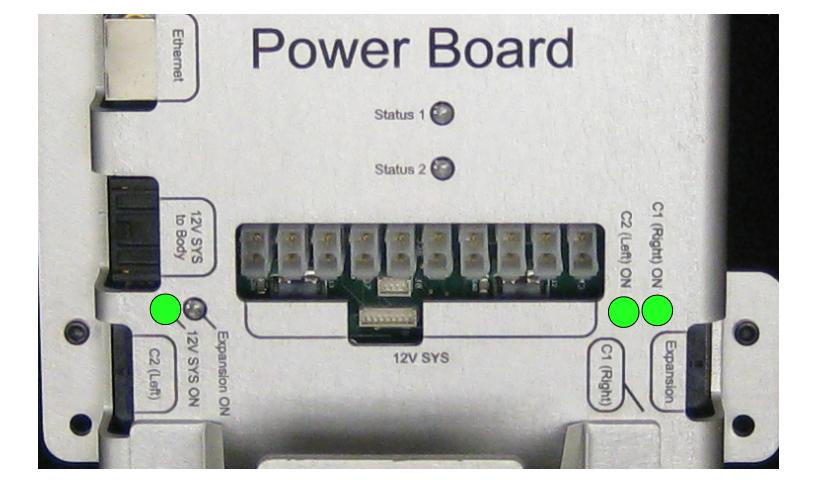
\includegraphics[scale=0.6]{pb_power1.jpg} 

The Blue LEDs indicate the motor bus power is enabled. Blue indicates a voltage higher than the 18V standby. These LEDs can also be orange if the output state is in the standby state.
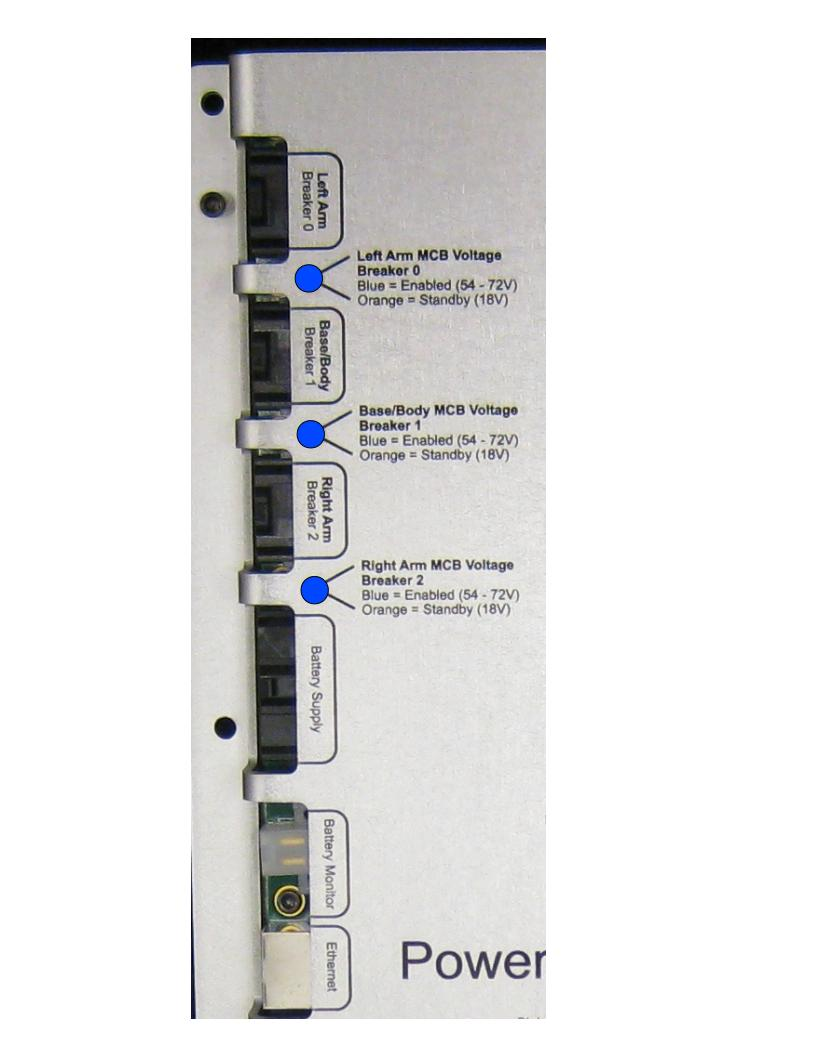
\includegraphics[scale=0.5]{pb_power2.jpg}

The status LEDs are used by the processor for debugging. In the event of a failure a status code will display on these LEDs. Someone must count the number of rapid blinks followed by a slight pause.
Status1 indicates the location where the fault occured and Status2 the cause of the fault.
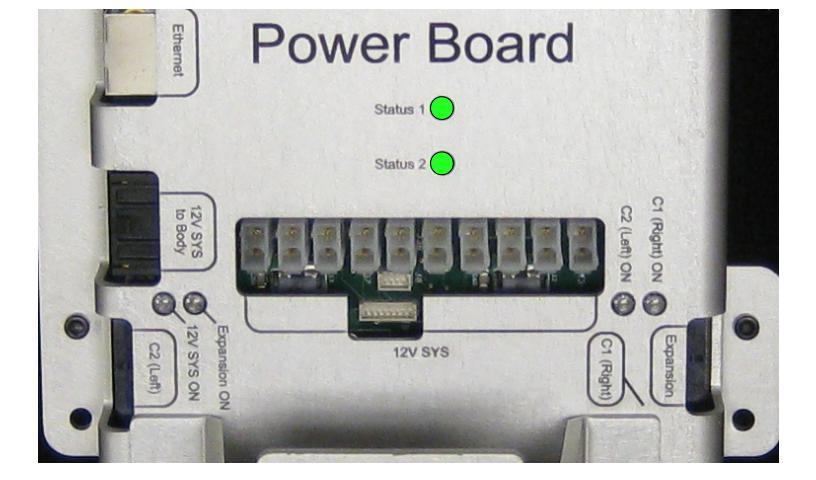
\includegraphics[scale=0.6]{pb_power3.jpg}

The following table provides some meaning for the error codes. For further diagnosis please provide the status codes in bug reports.

\begin{tabular}{|c|c|}
\hline
count & location \\
\hline
\hline
1 & Self Test \\
\hline
2 & Main Loop \\
\hline
3 & Breaker 0 \\
\hline
4 & Breaker 1 \\
\hline
5 & Breaker 2 \\
\hline
6 & Calibration Test \\
\hline
\end{tabular}

\begin{tabular}{c|c|}
\hline
\multicolumn{2}{|c|}{Main Loop Message} \\
\hline
count &  message \\
\hline
\hline
1 & Under Voltage Lockout \\
\hline
2 & Over Temperature Lockout \\
\hline
3 & Under Current condition \\
\hline
4 & Over Current condition \\
\hline
5 & Failed Self Test \\
\hline
6 & 18v Failure \\
\hline
7 & Fan tachometer failure \\
\hline
8 & calibration CRC failure \\
\hline
9 & Battery voltage low  \\
\hline
& \\
\hline
\multicolumn{2}{|c|}{Circuit Message} \\
\hline
1 & Disable via software command \\
\hline
2 & Failed during turn on cycle \\
\hline
3 & Shutdown by E-stop \\
\hline
4 & Circuit breaker tripped  \\
\hline
\end{tabular}

\subsection{Power for sensors}
As mentioned previously, the power board provides a \emph{12V system bus}, that provides a well regulated 12V supply. The regulated 12V supply is the only supply designed for additions and expansion. This 12V supply is essentially always on once the Power board completes a self test. It is also monitored for undervoltage conditions and is fairly robust.


A few limitations should be followed when adding loads to the 12V user supply. This supply is already supporting the 2 Hokuyo scanners, 2 ethernet switches, the wireless AP and the E-stop receiver. Considering the loads and the supplies capabilities with some headroom this leaves 5A for expansion.\\

{\bf 5A limit on 12V expansion}\\

Access to the 12V accessory bus is available in several locations:\\

Inside the top head assembly.\\

{\bf insert picture}\\


In the upper back.\\

{\bf insert picture}\\


In the lower back, directly connecting to the power board.\\

{\bf insert picture}\\

Before something is connected to this bus, strongly consider if hot plugging is safe. If you are uncertain, the safest choice is to shut the power system off completely.\\

All 12V connectors in the robot use the same connector, a 2x1 Molex Mini-Fit Jr. The mating connector part number is {\bf 39-01-3022} or from Digikey {\bf WM1021-ND}. Pin one is negative and pin 2 is positive. Pin 2 is the pin closest to the latch.



\chapter{PR2 Computers}
This section covers the configuration of the computers and software that comes installed on the robot
\section{Computer hardware}
The PR2 has two computers, each with 24 Gb of random-access memory (RAM), 2
quad-core Nehalem processors, and two attached hard-drives.  The
motherboards are XXX from Rackable systems.  For more information
about the computers themselves, please see the user manual and
documentation at XXX (link to Rackable information).

Additionally, the PR2 ships with a basestation computer which
facilitates seamless communication with the PR2 when transitioning
between wired and wireless networks, and additionally helps in
a number of maintenance tasks.
\subsection{Computer 1 (c1)}
Computer 1 (c1) is physically located on the right side of the
robot. It is referred to as the master computer because it serves a
number of key roles for the computer infrastructure:
\begin{itemize}
\item c1 stores the operating system for both computers.  c2 cannot
  boot unless c1 has booted first.
\item c1 is connected to the PR2 ethercat network, and is the only
  computer that can perform motor control.
\item c1 provides routing for the rest of the robot when it is plugged
  in via the WAN port .
\item c1 provides routing for the rest of the robot when connected to
  another network via an openVPN tunnel
\item c1 provides DHCP services for other devices connected to the
  robot internal network.
\end{itemize}

c1's PCI slot is used for a 4-port ethernet card, giving it a
total of 6 ethernet ports. These are:
\begin{itemize}
\item \texttt{lan0 - lan3}: connection to internal robot network 
\item \texttt{wan0}: connected directly to WAN port on back of robot
\item \texttt{ecat0}: connected to robot ethercat network 
\end{itemize}

\subsection{Computer 2 (c2)}
Computer 2 (c2) is physically located on the left side of the
robot. It is sometimes referred to as the slave computer because it
netboots from c1.

c2 only has 2 ethernet ports, \texttt{lan0} and \texttt{lan1}, both of
which are connected to the internal robot network.

\subsection{Basestation}
The basestation is a Zareason xPC.  It is a dedicated
point of contact through which network traffic to the robot can be
routed.  It has 2 ethernet ports, \texttt{wan0}, on the motherboard,
is the primary ethernet port.  It is intended to be plugged into your
building network.  \texttt{lan0}, on the pci card is a dedicated port
for servicing the robot.  When necessary, this port should be plugged
directly into the robot service port.

When configured properly, it is important that the basestation is
visible on port \texttt{1194} both via your wired building network as
well as via your building wireless network.  This will likely require
assistance from your local network administrator.

\section{Networking}
The majority of communication between components onboard the PR2
happens via an onboard ethernet network, referred to as the ``robot
internal network.''  This onboard network can be accessed directly via
either wired connection (through the service port), or wireless
connection (through the WAP).  Additionally, the robot can be accessed
via the basestation through a VPN tunnel.
\subsection{Network segments}
There are a couple of different important network segments, outlined
here, and discussed in more detail in the section ``Network
Explanation'' below.
\begin{itemize}
\item \texttt{10.68.0.0/24}: Primary Robot Internal Network. The
  \texttt{10.68.0.0} subnet is the primary network used internally by
  the computers on the robot.  Both computers and the basestation have
  addresses on this subnet.  Additionally, many of the ethernet-based
  devices, such as the power board, are given addresses on this
  subnet.  The robot Service Port, and the cradlepoint ctr350 Wireless
  Access Point are directly connected to this network, allowing a user
  to easily put their laptop on the robot internal network.  c1, if
  booted, will give out IP addresses via DHCP in the range
  \texttt{10.68.0.100-10.68.0.199}.  Important addresses on this
  network:
  \begin{itemize}
  \item \texttt{10.68.0.1} - c1 (lan0)
  \item \texttt{10.68.0.2} - c2 (lan0)
  \item \texttt{10.68.0.5} - wifi-router
  \item \texttt{10.68.0.6} - basestation (lan0)
  \item \texttt{10.68.0.91} - c1-esms
  \item \texttt{10.68.0.92} - c2-esms
  \item \texttt{10.68.0.250} - wap
  \end{itemize}
\item \texttt{10.69.0.0/24}: Secondary Robot Internal Network.  The
  \texttt{10.69.0.0} network is a second internal subnet.  The cameras
  are given addresses on this subnet to partition traffic accross the
  computer's two network interfaces of the computers. This way, heavy
  network utilization by the cameras is less likely to interfere with
  more critical computer functions such as NFS.
  \begin{itemize}
  \item \texttt{10.69.0.11} - c1 (lan1)
  \item \texttt{10.69.0.12} - c2 (lan1)
  \end{itemize}
\item \texttt{10.68.X.0/24}: Robot VPN Network. The primarily role of
  the basestation is to function as a VPN server for the robot.  Each
  robot can be given a unique VPN subnet to facilitate the operation
  of multiple robots using a single VPN server.  The basestation can
  be configured to automatically forward relevant traffic from the
  building network into the VPN network, hiding this from the
  end-user.  However, if greater security is desired, the basestation
  can instead be configured to require users to be assigned a vpn key
  to access the robot VPN network.  Important addresses on this
  network:
  \begin{itemize}
  \item \texttt{10.68.X.1} - c1 (tun0)
  \item \texttt{10.68.X.2} - c2 (via c1:tun0)
  \item \texttt{10.68.255.1} - basestation (tun0)
  \end{itemize}
\end{itemize}
\subsection{Network Explanation}
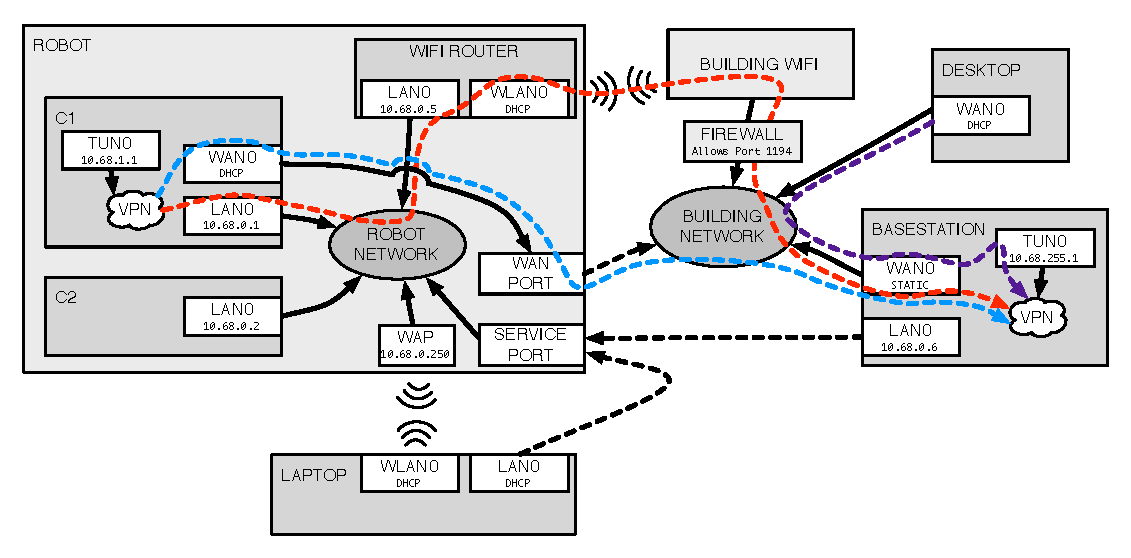
\includegraphics[width=400px]{images/pr2_network_diagram.pdf}

The above figure depicts the interaction between the robot and
building networks.  The dotted lines show paths which may or may not
be connected at any given point in time.  That is, the basestation or
a laptop may not always be plugged into the service port, and the
robot WAN port may not always be plugged into the building network.
The colored lines depict pathways that different network traffic
follows.  The main thing of importance to note is that there are three
ways to talk to the robot: direct wire, direct wireless, or VPN.
Additionally, the VPN traffic itself can be routed in one of two ways,
either via a wired or wireless path.
the VPN.  \textit{Note: for clarity, we have labeled all interfaces
  connected to the building network as WAN, and interfaces connected
  to the robot network as LAN, but this may well not be the case for
  laptops or desktops on your actual network, where the usual default
  interface name is typically ``eth0''}
\begin{itemize}
\item \textbf{Direct wired connection}.  One possibility is to connect
  a laptop, or the basestation \texttt{lan0} port to the robot service
  port.  This simply puts the laptop, or the basetation directly on
  the robot internal network.  The basestation is always configured to
  use the IP address \texttt{10.68.0.6}, whereas the laptop will
  likely be configured to use DHCP.  When plugged into the service
  port, you can talk to the robot LAN ports directly on the
  \texttt{10.68.0.0/24} subnet.  This system will work even if the VPN
  system is not functioning.  This is typically used for reinstalling
  the robot, or debugging other networking problems.
\item \textbf{Direct wireless connection}.  Another possibility is to
  connect a laptop directly to the robot WAP.  This is essentially
  identical to plugging into the service port.  The robot computers
  can be reached directly on the \texttt{10.68.0.0/24} subnet.
\item \textbf{VPN connection}.  When not plugged into the service
  port, the basestation and robot communicate over VPN.  The
  basestation acts as the VPN server, and is always reachable at
  \texttt{10.68.255.1}.  However, there are two mechanism through
  which the VPN traffic may be routed.
  \begin{itemize}
  \item \textbf{Wired VPN connection}. The wired VPN connection is
    depicted in blue.  This only occurs when the robot WAN port is
    plugged into the building network.  Note that \texttt{wan0} on c1
    goes directly to the robot WAN port.  When this is plugged into
    the building network, c1 acquires an IP address via DHCP.  At that
    point c1 initiates a connection to the basestation using a
    specified static IP address.  Once this connection is established,
    all vpn traffic is routed through this pathway.
  \item \textbf{Wireless VPN connection}.  The wireless VPN connection
    is depicted in red.  If the WAN port is not plugged in, the robot
    falls back on its wireless connection.  A secondary route instead
    sends traffic through the wifi-router, which must be configured to
    connect to the building wireless network.  In many cases, the
    wireless network is located outside the firewall, so it is
    important that the static IP of the basestation resolves properly
    and is allowed through the firewall on port 1194.
  \end{itemize}
  Regardless of how the robot is connected to the basestation, a
  desktop situated on the building network will always talk to the
  robot in the same way.  Traffic from the desktop, depicted in green,
  is actually routed through the basestation and into the VPN tunnel.
  Once in the tunnel, which pathway the robot is using is abstracted
  and the traffic seamlessly emerges from the other side of the
  tunnel.
\end{itemize}

\subsection{Service Port} The robot service port is the bottom
ethernet port on the back panel of the robot.  It connects directly to
the robot internel network, allowing you to connect to the computers
directly.  \textit{DO NOT PLUG THIS PORT INTO YOUR BUILDING NETWORK.}
c1 serves DHCP for this network and if it conflicts with another DHCP
server this will most likely cause problems both on your building
network and on the robot network depending on which DHCP server takes
precedence.
\subsection{WAN port} The robot WAN port is the top ethernet port on
the back panel of the robot.  This connects directly to \texttt{wan0}
on c1.  This port is intended to be plugged into your building
network.  The robot will attempt to acquire an IP address via DHCP,
and then attempt to contact the basestation at a known IP address.
\subsection{Wireless access point} The robot comes configured with a
cradlepoint ctr350 configured as a Wireless Access Point (WAP)
\href{http://www.cradlepoint.com/products/ctr350-mobile-broadband-router}.
The ESSID of this network defaults to ``<ROBOTNAME>\_LAN'', and allows
direct access to the Robot Internal Network.  You can configure the
WAP by plugging into the robot service port and going to the IP
address: \texttt{10.68.0.250}.  The default login and password are
``root'', ``willow.''

\subsection{Wireless router}
The PR2 has a
\href{http://www.linksysbycisco.com/US/en/products/WRT610N}{Linksys
  WRT610N} dual-N band wireless router.  This router can be configured
to connect to your building wireless network.  In the absence of a WAN
connection, the robot will attempt to contact the basestation through
this wireless router instead. You can configure the wireless router by
plugging into the robot service port and going to the IP address:
\texttt{10.68.0.5}.  The default login and password are ``root'',
``willow.''

\section{OS}
The operating system running on the PR2 computers is an extended
version of Ubuntu 9.04 (Jaunty Jackalope). It depends on a number of
additional packages for system configuration, but should otherwise be
familiar to for Ubuntu users. If you run into a computer problem not
covered by the PR2 documentation, the
\href{https://help.ubuntu.com/9.04/index.html}{Ubuntu Documentation}
is the next place to look.

\subsection{Networking}
To keep connections behaving sensibly when transitioning the VPN
connection to the basestation, the robot is configured to route ALL
traffic that is not on the robot internal network out through the
basestation.  This means that if VPN is not connected your robot will
not be able to see the outside world even though it might appear that
the network is configured appropriately.

This is handled using an \texttt{ip rule} configuration.  Most of
these rules are added by the init-script:
\texttt{/etc/init.d/iprules.sh}.  If you need to temporarily disable
the rule preventing traffic from going anywhere but the basestation,
you can manually remove the rule:

\begin{verbatim}
pr2admin@c1$ sudo ip rule del priority 3000
\end{verbatim}

This may be useful to do when repairing a system in a particularly bad
state since otherwise you may not be able to fetch necessary software
updates or download necessary configuration files.

\subsection{NFS and Unionfs}
The single largest difference between a normal Ubuntu installation and
the PR2 configuration is that c2 mounts nearly its entire filesystem
via NFS.  The exceptions to this are the directories \texttt{/etc},
\texttt{/var}, and \texttt{/pr2bin} which are mounted via
unionfs-fuse.  In short, unionfs allows one to specify an additional
overlay on top of the underlying filesystem.  The contents of this
overlay can be found in the directory \texttt{/slave} on c1.  Files
added here will show up in the appropriate location on c2.  For more
information on how this is set up, see the man page for
\texttt{unionfs-fuse} and look at the init-script
\texttt{/etc/unionfs-fuse-nfs-root}.

New software and configuration changes should only be made on c1.
Since c2 mounts most of its filesystems read-only, this will usually
be enforced for you.  If you are using a non-standard piece of
software that attempts to write to the filesystem outside of your home
directory you will likely need to make accommodating changes to either
the computer configuration or the software you are trying to run.

\subsection{autofs}
Both of the computers have automount configured for mounting the
\texttt{/home} partition of the other computer in a
computer-independent way using autofs. These automounts are located in
the directory \texttt{/pr}. To get to the home partition on c1 you can
use the path \texttt{/pr/1/} and to get to the home partition on c2
you can use the path \texttt{/pr/2/}. You should rarely need to do
this explicitly, but it is necessary to make sense of home directory
locations.

\subsection{Home directories}
The default configuration for user home directories (as given in
\texttt{/etc/passwd}) is \texttt{/u/username}.  Instead of a
directory, this location is by default a symlink to
\texttt{/pr/1/username} (locating the home directory on c1).  To place
a users home directory at a different location, such as the disk on
c2, an admin can simply move (or copy) the home directory and update
the symlink accordingly.

\subsection{Kernel}
Discuss RT\_PREEMT and anything else non-vanilla about the kernel.
(BLAISE HAS AGREED TO FILL THIS IN).

\subsection{Storage}
Each computer has two hard-drives - one internal 2.5" 500Gb
\href{http://www.seagate.com/www/en-us/products/laptops/momentus/momentus_7200.4_g_force/}{Seagate
  Momentus} drive, and a slot for a removable 3.5" SATA hard-drive
that is exposed on the top of the robot base.

By default the only hard-drive used is the internal drive on c1.
There are 3 relevant partitions created during installation:
\begin{itemize}
\item \texttt{c1:/dev/sda1} -- \texttt{/} -- holds the root filesystem
  for the OS
\item \texttt{c1:/dev/sda5} -- \texttt{c1:/home} -- stores user home
  directories (linked to from \texttt{/u} by way of \texttt{/pr/1})
\item \texttt{c1:/dev/sda6} -- \texttt{/hwlog} -- stores hardware logs
  generated by the pr2
\end{itemize}

The internal hard-drive on c2 has a single partition, which is
generally used as extra user storage:
\begin{itemize}
\item \texttt{c2:/dev/sda1} -- \texttt{c2:/home} -- stores user home
  directories (linked to from \texttt{/u} by way of \texttt{/pr/2})
\end{itemize}

Finally, both computers are configured to conveniently make use of the
additional removable drives.  Any drive loaded into the removable bay
should always show up as \texttt{/dev/removable}.  The mount point:
\texttt{/removable} is set up to allow users to mount the first
partition on this drive.
\begin{itemize}
\item \texttt{/dev/removable1} -- \texttt{/removable} -- stores
  temporary data users may want to move off the robot, primarily used
  for large bag files.  This is NOT mounted by default.  To use a
  driver users must explicitly
\begin{verbatim}
user@c1$ mount /dev/removable
\end{verbatim}
to use it, and should 
\begin{verbatim}
user@c1$ umount /dev/removable
\end{verbatim}
when done.  Until the drive is unmounted, you do not have a guarantee
the data has been written to disk, and if the robot runs out of
batteries, your data may be lost.
\end{itemize}

\subsubsection{Formatting Drives}
If you want to partion / reformat one of the removable drives, or the
the internal drive on c2, you can use the \texttt{formatdisk} helper
utility.  Simply pass it the name of the drive you want to format, for
example:
\begin{verbatim}
pr2admin@c2$ sudo formatdisk /dev/sda
\end{verbatim}
or
\begin{verbatim}
pr2admin@c1$ sudo formatdisk /dev/removable
\end{verbatim}

\subsection{Default user account}
The default account on the robot is ``pr2admin''.  When the robot is
first installed, it does not have a password set, however, this
password is set as part of the branding process.  When you first
receive the PR2 from Willow Garage the password will most likely be
set to ``willow''.

\subsection{Creating user accounts}
The expectation is that each person logging into the robot to develop
code will have their own user account.  Any robot admin can create a
new user using the
\texttt{\href{http://unixhelp.ed.ac.uk/CGI/man-cgi?adduser}{adduser}}
command (NOT the \texttt{useradd} command), on c1.  User accounts are
automatically mirrored on c2.

Some examples:
\begin{verbatim}
pr2admin@c1$ sudo adduser bob
pr2admin@c1$ sudo adduser bill --shell /usr/bin/tcsh --uid 2000
\end{verbatim}

\textit{Note: it may be helpful to assign users the same UID used on
  your building network so the UIDs are consistent when mounting shares
  or moving around the removable drives.}

Moving the home directory and creating the symlink is handled for you
by the script: \texttt{/usr/local/sbin/adduser.local}, which gets run
automatically as a part of user-creation.  You should not need to
worry about this script at all unless you are changing the
user-creation process.

\subsection{User groups}
There are a couple of important groups on the pr2:
\begin{itemize}
\item \texttt{admin} -- Members of this group have full root privileges when using the sudo command
\item \texttt{rosadmin} -- Members of this group have access to change ros-specific configuration settings in \texttt{/etc/ros}
\item \texttt{apt} -- Members of this group can install new software
\end{itemize}

To add a user to a group, use the
\texttt{\href{http://unixhelp.ed.ac.uk/CGI/man-cgi?usermod}{usermod}}
command.  The most common invocation uses the options \texttt{-a}
(append) and \texttt{-G} (group).  For example:

\begin{verbatim}
pr2admin@c1$ sudo usermod -a -G admin bob
\end{verbatim}

\subsection{Backing up and restoring users}
Before reinstalling the robot operating system you will likely want to
back up the user accounts. This can be done with the command:
\texttt{pr2-usermigrate}. To save users:
\begin{verbatim}
pr2admin@c1$ sudo pr2-usermigrate save myrobot.users
\end{verbatim}

Move this file off the robot before reinstalling.  Then, to restore users:
\begin{verbatim}
pr2admin@c1$ sudo pr2-usermigrate load myrobot.users
\end{verbatim}

\subsection{Clock synchronization}
Consistent time-stamping of data from the two computers is important
for interpreting sensor data on a moving system.  As a result, keeping
the system time on the two computers synced together requires some
attention.  The system that is used for this is
\href{http://chrony.tuxfamily.org/}{chrony}, and the general strategy
is to have the two computers tightly coupled to one another, but
loosely coupled to an external time source to prevent the robot time
from drifting too far from the outside world.

If you find your clocks in an inconsistant state, you may want to try
restarting chrony on the basestation, c1, and c2, in that order.
\begin{verbatim}
pr2admin@basestation$ sudo /etc/init.d/chrony restart
pr2admin@c1$ sudo /etc/init.d/chrony restart
pr2admin@c2$ sudo /etc/init.d/chrony restart
\end{verbatim}

\section{Basestation Setup and Pairing}
Before you can use the robot and basestation, it needs to be
configured.  This configuration can be done by logging into the
basestation.  The default account is ``pr2admin'' with password
``willow''.  The following instructions assume that the basestation is
plugged into the robot via the service port.

\subsection{Requirements}

\subsubsection{Naming}
It order for ROS to work properly, it depends on each computer in your
system being able to correctly resolve the hostnames of all other
computers in your ROS system.  For an in depth explanation, please
familiarize yourself with
\href{http://www.ros.org/wiki/ROS/NetworkSetup}{http://www.ros.org/wiki/ROS/NetworkSetup}.
However, in short, you are probably going to need 3 hostnames, and 3
IP addresses -- one for the basestation, and one for each of the two
robot computers.  Each of these 3 hostnames MUST either be resolved by
your building network DNS server, or else they will need to be added
to the \texttt{/etc/hosts} file of all the relevant computers.

\subsubsection{IP Address configuration}
For the robot to be able to find the basestation, it needs to be given
a constant IP address.  Unless you have a reason not to, this IP
address should be assigned to the basestation statically.  However, if
you are certain that your DHCP server will always assign the same IP,
it is ok for this IP to be assigned via DHCP.

The IP address assigned to your basestation must be visible on both
the wired and wireless segments of your building network on port
\texttt{1194}.  This is the port that VPN uses when the robot makes
its connection back to the basestation (it can be changed by modifying
\texttt{/etc/openvpn/server.conf} on the basestation).  Depending on
how secure your network is, and whether these segments are separated
by a firewall, you may need assistance from your local sysadmin to
allow traffic through on this port.

Finally, for the robot to be able to find the basestation, both the
wired and wireless networks must provide a DHCP server.  The operation
of the system is that the robot will acquire an IP address via DHCP
and then contact the basetation at the known IP address that it is
paired to.  Review the section on Networking for a more thorough
overview.

\subsubsection{Examples}

In the remainder of the examples in this section we will assume that
our basestation has been given the hostname \texttt{prbase1}, and our
computers will be named \texttt{prx1} and \texttt{prx2}.  We assume
that DNS resolves them correctly as follows:

\begin{itemize}
\item \texttt{prbase1} -- \texttt{192.168.1.100}
\item \texttt{prx1} -- \texttt{192.168.1.101}
\item \texttt{prx2} -- \texttt{192.168.1.102}
\end{itemize}

\subsection{Plugging things in}
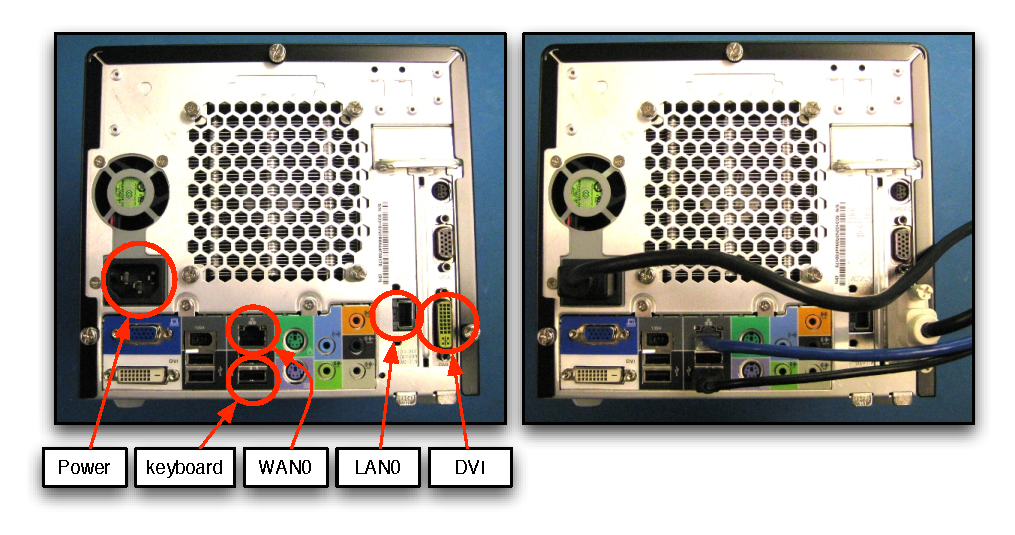
\includegraphics[width=350px]{images/pr2_basestation_plugs.pdf}

When plugging in the basestation, make sure that you plug WAN0 (on the
motherboard) into your building network.  LAN0, on the PCI card, is
only intended to be plugged into the robot service port.

Additionally, it is important to plug the DVI port into the installed
graphics card (on the right side of the computer) and not the extra
DVI port on the motherboard.

There is only one place to plug in the power, and your keyboard/mouse
can be plugged into any of the available USB ports.

\subsection{Configure the Basestation Network}

There are two ways to set up the basestation, using a static IP, or
DHCP.  It is strongly recommended that you use a Static IP unless you
have a very good reason to use DHCP and understand configuring your
DHCP server to obey client-id-based requests.

\subsubsection{Static IP}

To configure the basestation with a static IP, you must edit the file
\texttt{/etc/network/interfaces} and change \texttt{wan0} to use a staic ip
address, for example:
\begin{verbatim}
iface wan0 inet static
      address 192.168.1.100
      netmask 255.255.255.0
      gateway 192.168.1.1
      post-up robot-forward start
      pre-down robot-forward stop
\end{verbatim}
You will also need to update \texttt{/etc/resolv.conf} to contain the
appropriate nameserver, e.g.,
\begin{verbatim}
domain school.edu
search school.edu
nameserver 192.168.1.1
\end{verbatim}

\subsubsection{DHCP}
If you are using DHCP, you must make sure that your DHCP server
respects the client-id specification and is configured to assign a
consistant IP address to the client-id of the basestation.
\textit{NOTE: macaddress based assignment of IPs will not work
  correctly because the basestation also acquires IPs on behalf of the
  robot.}  The default client-id for the basestation is
``basestation.''  If you need to change this to a different client-id,
you must edit the file \texttt{/etc/dhcp3/dhclient.conf}, and change
the relevant line, for example
\begin{verbatim}
send dhcp-client-identifier "prbase1";
\end{verbatim}

\subsubsection{Hostname}
You will also likely need to change the hostname of the basestation.
Leaving it as ``basestation'' is ok, but you need to make sure the DNS
server correctly resolves this name to the IP address you have
assigned the basestation.  To change the hostname you will need to
edit the files: \texttt{/etc/hostname}, to just contain the name of
the basestation.  For example:
\begin{verbatim}
prbase1
\end{verbatim}
and edit \texttt{/etc/hosts} to resolve the basestation locally.
After modifying, \texttt{/etc/hosts} it should look something like:
\begin{verbatim}
127.0.0.1       localhost
127.0.1.1       prbase1.willowgarage.com        prbase1

# The following lines are desirable for IPv6 capable hosts
::1     localhost ip6-localhost ip6-loopback
fe00::0 ip6-localnet
ff00::0 ip6-mcastprefix
ff02::1 ip6-allnodes
ff02::2 ip6-allrouters
ff02::3 ip6-allhosts

### The following lines were added automatically by pr2-basestation ####
10.68.0.1 c1
10.68.0.2 c2
### The preceeding lines were added automatically by pr2-basestation ###
\end{verbatim}
Finally, you need to actually set the hostname using the hostname command, for example:
\begin{verbatim}
pr2admin@basestation$ sudo hostname prbase1
\end{verbatim}

\subsubsection{Applying Settings}
Once you have reconfigured the network, you should reboot the
basestation to make sure the network comes back up correctly.

\subsection{Configure the Robot Wifi}
The Linksys wrt610n on the robot is located at the IP address:
\texttt{10.68.0.5}. To configure it, either plug a laptop or a
basestation into the robot service port, open a web-browser and go to:
\texttt{http://10.68.0.5}.  Click on the ``Wireless'' tab.  The
default login should be ``root'' and ``willow,'' although after a
factory reset the router may end up with login, ``root'' and
``admin''.  Set either ``Wireless Physical Interface wl0'' (for 2.5
Ghz) or ``Wireless Physical Interface wl1'' (for 5 Ghz) to client mode
and enter the SSID for your network.  If you need to change other
settings, make sure that under ``Setup,'' the WAN connection type is
``Automatic Configuration - DHCP'', the local IP Address is
\texttt{10.68.0.5}, and the DHCP Server is Disabled.  When you are
done, make sure you choose to ``Apply Settings.''

To test the setup of the wireless, you can temporarily add a route on
the basestation which will route a particular IP address through the
wifi router.
\begin{verbatim}
$ sudo ip route add 157.22.19.22 via 10.68.0.5 dev lan0
\end{verbatim}
Then point your web-browser to: \texttt{http://157.22.19.22}. This
should take you to the willowgarage home page.  

It may take a short time for the wireless router to connect to the
network. 

Once that is working, you should remember to disable the route so that
it works if the basestation is not plugged into the service port:
\begin{verbatim}
$ sudo ip route del 157.22.19.22 via 10.68.0.5 dev lan0
\end{verbatim}

\subsection{Initialize the Basestation VPN Server}
One of the primary functions of the basestation is to host a VPN
server that the robot can connect to.  The server needs an appropriate
key.  To generate the key for the VPN server run:

\begin{verbatim}
pr2admin@basestation$ sudo /etc/openvpn/gen_server_key
\end{verbatim}

It will prompt you for some information.  It is good practice to get
the information correct, but will not actually impact the performance
of the robot.

\subsection{Pairing with the Robot}

Robot pairing is performed with the the \texttt{robot-brand} command
on the basestation.  It takes 5 arguments:

\begin{itemize}
\item robotname -- This is the name your robot will be given.
\item c1name -- This is the intended hostname of c1.  Your DNS server needs to resolve this to the IP address you intend to use for your robot.
\item c2name -- This is the intended hostname of c2.  Your DNS server needs to resolve this to the IP address you intend to use for your robot.
\item VPN subnet -- Unless you are using multiple robots, this should be 10.68.1.0.  The 3rd field of the IP, however, can be any value other than 0 and 255, which are reserved for the robot local network and the basestation server respectively.  No two robots on the same basestation should be assigned the same VPN subnet.
\item Basestation IP -- This is the static IP address you have assigned to your basestation \texttt{wan0}.
  It is worth checking that it is correct using the \texttt{ifconfig} command:
\begin{verbatim}
pr2admin@basestation:~$ ifconfig wan0
wan0      Link encap:Ethernet  HWaddr 00:30:1b:48:c8:f8  
          inet addr:192.168.1.100  Bcast:192.168.1.255  Mask:255.255.255.0
          inet6 addr: fe80::230:1bff:fe48:c8f8/64 Scope:Link
          UP BROADCAST RUNNING MULTICAST  MTU:1500  Metric:1
          RX packets:2702 errors:0 dropped:0 overruns:0 frame:0
          TX packets:2709 errors:0 dropped:0 overruns:0 carrier:0
          collisions:0 txqueuelen:1000 
          RX bytes:129699 (129.6 KB)  TX bytes:218528 (218.5 KB)
          Interrupt:17 
\end{verbatim}
In this case the address is \texttt{192.168.1.100}.
\end{itemize}

To actually brand the robot, first plug the basestation into the
service port of the robot, and then use the robot-brand command

\begin{verbatim}
pr2admin@basestation$ sudo robot-brand <ROBOT_NAME> <C1_NAME> <C2_NAME> <VPN_SUBNET> <BASESTATION_IP>
\end{verbatim}

For example, if your robot were going to be named ``prx'', c1 was
going to named ``prx1'', c2 was going to be named ``prx2'', and your
basestation was located at \texttt{192.168.1.100}, you would run:

\begin{verbatim}
pr2admin@prbase1$ sudo robot-brand prx prx1 prx2 10.68.1.0 192.168.1.100
\end{verbatim}

During the branding process, it may prompt you for the password of
``root@c1''.  By default this will be ``willow''.  Additionally, you
may be prompted to choose a password for the pr2admin account.

When the script finishes, you should be able to connect to the robot
over the VPN.  Check that it works and then exit.
\begin{verbatim}
pr2admin@prbase1$ ssh pr2admin@10.68.1.1
pr2admin@prx1:~$ exit
\end{verbatim}

\subsection{Forwarding IPs to the robot}

To make contacting the robot from your building network more convenient,
the basestation can be configured to forward IP addresses (assigned
statically or via DHCP) to the robot.

To set this up, edit the file: \texttt{/etc/robot-forward.conf} and add the lines:

\begin{verbatim}
<C1_NAME> <VPN_SUBNET>.1 <ROBOT_IP1>
<C2_NAME> <VPN_SUBNET>.2 <ROBOT_IP2>
\end{verbatim}

For example, in our case we would use:

\begin{verbatim}
prx1 10.68.1.1 192.168.1.101
prx2 10.68.1.2 192.168.1.102
\end{verbatim}

Note that for this to work properly, we should have named our robot
computers prx1 and prx2, respectively, and furthermore our DNS server
should resolve ``prx1'' to \texttt{192.168.1.101}, and ``prx2'' to
\texttt{192.168.1.102}.

Much like the basestation, you can also have these IPs assigned via DHCP:

\begin{verbatim}
prx1 10.68.1.1 dhcp
prx2 10.68.1.2 dhcp
\end{verbatim}

In which case the basestation will use the client-id's ``prx1'' and
``prx2'' to acquire 2 IP addresses from the DHCP server.  These IPs
should be assigned consistantly given the client-id's, and should
match the IPs that the DNS server returns for the particular hostnames.  

Robot forwarding is enabled whenever the networking starts, but to
manually start forwarding, you can run:

\begin{verbatim}
pr2admin@prbase1$ sudo robot-forward start
\end{verbatim}

You should not be able to contact the robot at the IP address you have
given it, and, if your DNS server is set up properly, using it's
hostname.  For example:

\begin{verbatim}
pr2admin@prbase1$ ssh pr2admin@192.168.1.101
\end{verbatim}

and

\begin{verbatim}
pr2admin@prbase1$ ssh pr2admin@prx1
\end{verbatim}

If you need to disable forwarding you can run:

\begin{verbatim}
pr2admin@prbase1$ sudo robot-forward stop
\end{verbatim}

\section{Software Maintenance}

When the robots ship, the most recent version of ROS and the PR2
software stacks is installed in /opt/ros.  By default, new users will
have a ROS installation which references the pre-installed code.
Users who wish to modify or replace a part of the system are
recommended to install a development version of the stacks or packages
which they wish to modify, but to continue to use the base
installation for most of the robot functionality.

Debian packages exist for all of the custom software and
configurations on the robot.  The package which pulls in all the other
requirements is called \texttt{pr2-environment}.
\texttt{pr2-environment} depends on \texttt{pr2-core}, which in turn
depends on \texttt{ros-boxturtle-pr2}, the meta-package which contains
all of the ROS software for the PR2.

To upgrade the software on your robot, you can simply use \texttt{apt}:

\begin{verbatim}
$ sudo apt-get dist-upgrade
\end{verbatim}

Which will update all packages on your system, pulling in security fixes for
the pr2 configuration as well as for the appropriate ros-release.

\section{Reinstall the Basestation}
If you have a basestation USB installer, you can reinstall the
basestation to revert it to a completely fresh state.  Creating a new
USB installer is outside the scope of this manual, but instructions
for downloading and creating one can be found on the PR2 website.

\subsection{Booting off the USB installer}
To boot off the USB installer:
\begin{itemize}
\item Insert the USB stick into one of the USB ports in the basestation
\item Reboot the basestation
\item Press the \texttt{<DEL>} key to enter setup
\item Choose ``Advanced BIOS Features''
\item Choose ``Hard Disk Boot Priority''
\item Select the drive listed as ``USB-HDD0'' and hit ``Page Up'' to make it number 1
\item Hit ``F10'' to save and exit the setup
\item The computer should boot off of the USB stick.
\item If the installer complains about not being able to find the ISO, hit ``Enter'' to continue, twice and the installation should continue.
\item When the installer completes, hit ``Enter'' to shut down and remove the USB stick.
\item When the basestation boots you should have a fresh image -- consult the section on Basestation Setup and Pairing to configure the basestation.
\end{itemize}

\section{Reinstall the Robot}

To reinstall the robot, first back up anything you need off of c1.
Next, shutdown the comptuers using \texttt{pr2-shutdown --netboot}.

You must then plug the service port directly into the basestation.
You can then run the robot installer:

\begin{verbatim}
pr2admin@basestation$ sudo robot-install
\end{verbatim}

Boot c1 by pushing the power button with a paperclip.

After N minutes, the netconsole on the basestation will show the
install dialog.  Hit enter to start the installer and wait for it to
complete.

Once the installer has completed and the robot is shut down, you can
boot it up.  You will now need to pair it with the basestation before
you can use it.

\subsection{Forcing netboot}

If the robot BIOS is not configured to netboot, you might need to be
able hit f12 on the keyboard.  You can do this in one of two ways.

The easier way to to connect up to the KVM.  (See section XYZ on connecting to the KVM.)

Alternatively, plug a keyboard into the PR2.  This can be done using
the aux usb port under the back cover.  To remove this cover, follow
the instructions in section XYZ.

When the robot is booting you will hear 2 beeps followed by a short
pause, and then another 2 beeps.  After the 4th beep, hit f12 on the
keyboard (either physically or through the KVM) to force c1 to netboot.


\chapter{Running the PR2}
Running the PR2 requires a basic understanding of ROS (\href{http://www.ros.org}{http://www.ros.org}), the BSD-licensed 
Robot Operating System.  A ROS system consists of multiple processes running on multiple computers.  If you are not 
familiar with ROS, it is highly recommended that you follow some of the \href{http://www.ros.org/wiki/ROS/Tutorials}{beginner tutorials} 
on ros.org. Familiarity with ROS tools will make using the robot much easier.  In particular, you should understand 
what a launch file is and how to run it, and how to run ROS with nodes on multiple computers. This chapter will walk 
you through starting up and running a PR2, using ROS.

\section{Getting set up}
\subsection{Out of the box}
If you are starting your PR2 for the first time at your institution, please read the previous sections,\ref{Setting up PR2 in your lab}.  
This will give you advice on setting up the network, setting the administrative password, and picking a safe location for 
charging the PR2.  This chapter assumes that the PR2 is already set up for your lab.
\subsection{Batteries and power}
Before running the robot, you need to make sure it has power.  The battery life of the PR2 is approximately two hours, 
so it is a good idea to keep the PR2 plugged in when not in use.  You can follow the instructions in this chapter to start up 
the PR2 while it is plugged into the power outlet, which will keep the batteries charged.
\subsection{Run-stop}
The PR2 will not run its motors unless both run-stop buttons (the red push-button on the middle of the PR2's back, and 
the yellow wireless run-stop transmitter) are enabled.  Before you operate the PR2, you should have the wireless run-stop 
nearby, so that you can shut down the motors if you need to.  Before turning on the robot, press the red ``stop'' button on the 
wireless run-stop transmitter to prevent the motors from moving before you are ready.

%Add image of red push-button on PR2's back here
\begin{figure}[h]
\centering
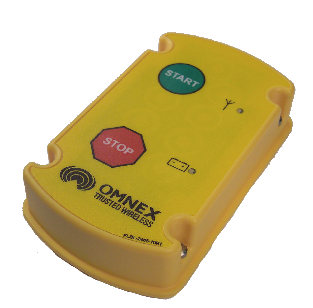
\includegraphics[width=150px]{run_stop.png}
\caption{The PR2 wireless run-stop.}
\label{fig:runstop}
\end{figure}

The wireless run-stop also uses battery power, which can run down. Therefore, it is a good idea to turn the wireless run-stop off when not in use. If the wireless run-stop runs out of battery charge, then the battery light (the light next to the battery symbol in the lower half of the wireless run-stop face) will flash. To change the battery, you will need a slotted screwdriver to open the wireless run-stop case and replace the batteries.

\begin{figure}[!h]
\centering
\includegraphics[width=125px]{opening_runstop.png}
\caption{Opening the PR2 wireless run-stop to change the batteries.}
\label{fig:opening-runstop}
\end{figure}

\subsection{Getting an account}
Before using the PR2, you will also need an account on the robot computers.  If you try to log in to the robot and the 
robot administrator has not created an account for you on the robot yet, then you will see:
\begin{verbatim}
Permission denied, please try again
\end{verbatim}
when you try to log in to the robot. Ask the robot administrator to create an account for you, using the instructions 
in section \ref{creating accounts}.
\section{Turning PR2 on}
To turn the PR2 on, you should first verify that the wireless run-stop is off. On the wireless run-stop, press the 
red button, and make sure there are no flashing lights on the wireless run-stop. Then switch the red DC breaker on 
the back panel of the robot to the ``on'' position.  

\begin{figure}[h]
\centering
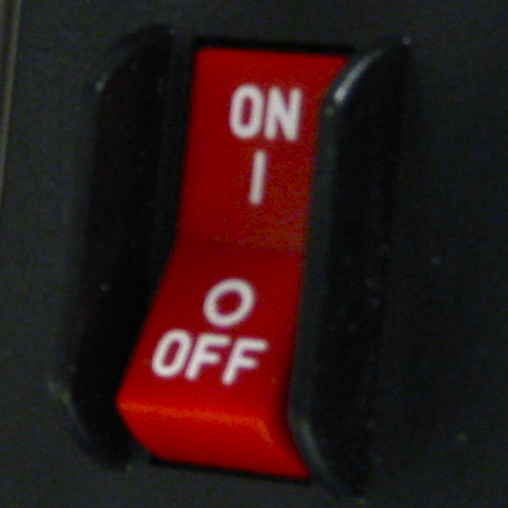
\includegraphics[width=50px]{dc_breaker.png}
\caption{The PR2 DC breaker switch in the ON position.}
\label{fig:dc_breaker}
\end{figure}

You should see the red lights on the computers turn on, hear the fans spin up, and hear several rising-tone beeps from the computers 
as they boot.  The process of booting the computers will take about 5 minutes.  If the robot is already running, you can 
skip this step (but should still disable the wireless run-stop).
\subsection{Logging in}
Once the robot is on, \texttt{\href{http://unixhelp.ed.ac.uk/CGI/man-cgi?ssh}{ssh}} into the main computer using the account 
created for you by the administrator. 

In the following tutorial, we will use pr\textcolor{red}{x}1 to refer to the first computer on robot \textcolor{red}{x}.  
Ask your robot  administrator what name you should use for the robot you want to run. To log in to the robot, type
\begin{verbatim}
$ ssh username@prx1
\end{verbatim}
You will notice that you are already set up with a ROS environment.  To see what packages are available to you, type
\begin{verbatim}
$ rospack list-names
\end{verbatim}
and you should see a list of the ros packages currently in your path.

\subsection{Checking for other users}
If you logged in to a robot that was already running, you should check to see if anyone else is using the robot. To 
find out who else is using the robot, type
\begin{verbatim}
$ ckill list
\end{verbatim}
This will show you what programs are currently running on the robot.  If other people have processes running on the 
robot, you will need to find out if you can interrupt their work. You should find out who is on the robot and ask them 
to allow you to kill their processes so that you can work on the robot.  If you cannot find the people running processes 
on the robot, ask the robot adminstrator for guidance on what the policy is in your lab. If it is fine for you to kill 
the other processes running on the robot, you can type
\begin{verbatim}
$ sudo robot stop
\end{verbatim}
and all the processes that are being run on the robot will be killed.
\section{Starting the software}
The launch file /etc/pr2/pr2.launch is used to start up the basic functionality of the robot.  This includes drivers for 
the sensors, motors, speakers, projector, power system, and joystick as well as the default set of realtime controllers, 
processing and logging of diagnostics information, and monitors for various types of problems your robot could experience.  On a new robot, this launch file is standard, but if the robot you are working on has been altered (e.g., has additional sensors, has only one arm), then it is likely that someone administering the robot has also updated the /etc/pr2/pr2.launch file to work with your robot's configuration.

Once you are logged in and ready to start the robot, you can run the robot by typing
\begin{verbatim}
$ robot start
\end{verbatim}
If this does not work, try typing
\begin{verbatim}
$ sudo robot start
\end{verbatim}
Running robot start will start the roslaunch for you in the background as a system user. This will 
allow you to continue to use your current terminal and the robot will keep running after you log out.  

If you used ``robot start'' then you will not need to open a new terminal to complete other commands. You can type 
\begin{verbatim}
$ rostopic list
\end{verbatim}
to see the topics being published by the system. 

Alternatively, if you prefer to see everything that is going on, you can run the roslaunch manually, but you will need to keep that 
window open until you are done using the robot. Closing that the terminal in which you roslaunched will terminate the 
roslaunch.
\begin{verbatim}
$ roslaunch /etc/pr2/pr2.launch
\end{verbatim}
to start up the pr2.  

If you used ``roslaunch'' to start the robot, then you will need to open a new terminal and type
\begin{verbatim}
$ ssh username@prx1
$ rostopic list
\end{verbatim}
to see what topics are being published by the system in the new terminal while the roslaunch continues to run in the 
original terminal. Remember that \textcolor{red}{x} is a placeholding variable to be replaced with your robot's ID.

Either way, the robot should be running, but since you have the wireless run-stop disabled, the motors will not be moving.  

\section{Running the dashboard}
When running the robot, the pr2\_dashboard should always be up on your screen.  This is how the robot software will 
let you know if something is going wrong, and is also how you turn the motors and power on and off.  

On a computer with a built ROS installation (e.g., the base-station desktop computer that ships with the robot), not on the robot itself, set your ROS\_MASTER\_URI to point at the master running on the robot and launch the dashboard by typing
\begin{verbatim}
$ export ROS_MASTER_URI=http://prx1:11311
$ rosrun pr2_dashboard pr2_dashboard
\end{verbatim}
You should see the pr2\_dashboard control panel (a graphical user interface) appear and provide you with information about the state of the robot. It is ok if not all of the icons are green. In fact, the Runstops should be ``warning'' you that the wireless runstop is not on. 

If you do not see the pr2\_dashboard control panel appear, then there is a chance that you have not yet ``made'' the pr2\_dashboard. To do this, type
\begin{verbatim}
$ roscd pr2_dashboard
\end{verbatim}
to navigate to the pr2\_dashboard directory. Then type
\begin{verbatim}
$ rosmake pr2_dashboard
\end{verbatim}
to make pr2_dashboard.

Take a moment to review the state of the robot. You can get a sense for the health of 
your robot by looking at the diagnostics information; click on the wrench on the far left.  Since you have the run-stop disabled, you see that the motors are giving you a warning (CURRENTLY THIS IS AN ERROR.  SHOULD CHANGE TO WARNING BY 
ROBOT SHIP DATE).  You should see a warning because the robot was just turned on and the encoders on the joints have not 
been calibrated yet.

If you see warnings or errors in any other sections, you should read the error messages and try to figure out what the 
problem is.  Ask your robot administrator for help if there are errors that you do not understand.
\subsection{Understanding pr2\_dashboard}
When running the PR2, the most important piece of software for you to understand and control the state of the system is 
the pr2\_dashboard. pr2\_dashboard, Figure~\ref{fig:dashboard}, is a GUI for debugging and controlling low-level state 
of the PR2. The dashboard displays the diagnostic, circuit breaker, run-stop, and battery status.
\begin{figure}[h]
\centering
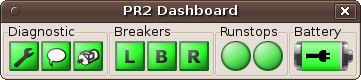
\includegraphics[scale=0.5]{pr2_dashboard.png}
\caption{The PR2 dashboard.}
\label{fig:dashboard}
\end{figure}
\begin{description}
\item[Diagnostic Status] The state of the robot is shown by the diagnoctic indicators in the pr2\_dashboard. \\

    \newcolumntype{S}{>{\centering\arraybackslash} m{.9cm} }%
    \begin{tabular}{m{6cm}SSSS}
    Component & OK & Warn & Error & Stale\\
    &&&&\\
    Diagnostics: Clicking pops up the Robot Monitor & 
\includegraphics[scale=0.5]{diag_ok.png}&
\includegraphics[scale=0.5]{diag_warn.png}&
                                                      
\includegraphics[scale=0.5]{diag_error.png}&
\includegraphics[scale=0.5]{diag_stale.png}\\
    &&&&\\
    Rosout: Clicking pops up rxconsole & 
\includegraphics[scale=0.5]{rosout_ok.png}&
\includegraphics[scale=0.5]{rosout_warn.png}&
                                        
\includegraphics[scale=0.5]{rosout_error.png}&
\includegraphics[scale=0.5]{rosout_stale.png}\\
    &&&&\\
    Motors: Clicking allows you to halt or reset motors & 
\includegraphics[scale=0.5]{motor_ok.png}& N/A &
                                                          
\includegraphics[scale=0.5]{motor_error.png}&
\includegraphics[scale=0.5]{motor_stale.png}\\
   \end{tabular}

\item[Circuit Breaker Status] The circuit breakers are labeled L/B/R, which stand for Left Arm, Base/Spine, and Right Arm. 
Each breaker can be in one of four states, and clicking on any of the breakers will pop up a menu (Figure~\ref{fig:breaker_menu}), allowing you to change the state of one or all of them:
\begin{figure}[h]
\centering
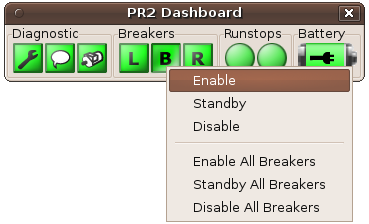
\includegraphics[scale=0.5]{breakers_menu.png}
\caption{The circuit breaker options menu.}
\label{fig:breaker_menu}
\end{figure}

    \newcolumntype{S}{>{\centering\arraybackslash} m{1.7cm} }%       
    \begin{tabular}{m{2.6cm}SSSS}
     & Enabled & Standby & Disabled & Stale\\
    Breaker Status & 
\includegraphics[scale=0.5]{L_ok.png}
\includegraphics[scale=0.5]{B_ok.png}
\includegraphics[scale=0.5]{R_ok.png}&
                     
\includegraphics[scale=0.5]{L_stby.png}
\includegraphics[scale=0.5]{B_stby.png}
\includegraphics[scale=0.5]{R_stby.png}&
                     
\includegraphics[scale=0.5]{L_dis.png}
\includegraphics[scale=0.5]{B_dis.png}
\includegraphics[scale=0.5]{R_dis.png}&
                     
\includegraphics[scale=0.5]{L_stale.png}
\includegraphics[scale=0.5]{B_stale.png}
\includegraphics[scale=0.5]{R_stale.png}\\
   \end{tabular}



\item[Runstop Status] The runstop indicators display the status of the PR2 runstops and their states cannot be changed using the dashboard. 
There are two run-stops on the robot, a wireless run-stop, see \ref{wirelessrunstop}, and a red push button run-stop on the back of the robot.\\

    \newcolumntype{S}{>{\centering\arraybackslash} m{2.5cm} }%                                                                                                         
    \begin{tabular}{m{2.6cm}SSS}
     & OK & Physical Stop is Off & Wireless Stop is Off\\
    Runstop Status & 
\includegraphics[scale=0.5]{runstop-green.png}
\includegraphics[scale=0.5]{runstop_wireless_ok.png}&
                     
\includegraphics[scale=0.5]{runstop-red.png}\includegraphics[scale=0.5]{runstop_wireless_ok.png}&
                     \includegraphics[scale=0.5]{runstop-yellow.png}\includegraphics[scale=0.5]{runstop_wireless_stop.png}\\
   \end{tabular}

Now you can enable the wireless run-stop by pressing the green "START" button on the wireless run-stop. If this works properly, then you should see the robot run-stop icon turn green in the dashboard.

\item[Battery Status]
The battery will change its color and \% filled based on the amount of battery remaining. It will also show a power-plug symbol if the robot is charging.
    \newcolumntype{S}{>{\centering\arraybackslash} m{1.85cm} }%                                                      
                                                                                                                      
    \begin{tabular}{m{2.5cm}SSSS}
     & $>$ 50\% & 30 - 50\% & $<$ 30\% & Charging\\
    Battery Status & \includegraphics[scale=0.5]{battery_green.png}&
                     \includegraphics[scale=0.5]{battery_yellow.png}&
                     \includegraphics[scale=0.5]{battery_red.png}&
                     \includegraphics[scale=0.5]{battery_charging.png}\\
   \end{tabular}


\end{description}

\section{Calibrating the joints}
If you do not discover any problems in the diagnostics, and you want to continue with robot bringup, press the green 
button on the wireless run-stop.  This should change the state of the run-stop indicator on the dashboard to a green 
circle, and will allow the robot to turn power on for the motors.  The next step is to enable the circuit breakers 
(marked L, B, R).  When you click on the circuit-breaker icon, select ``enable all'' from the menu to turn on all 
three breakers.

Finally, check that the area around the robot is safe for it to move its arms, click on the picture of a motor, and 
select ``reset motors.''  When you do this, the robot will move its joints to find the absolute reference positions of 
each joint so that it can calibrate the mechanism.  When calibration is finished, you should see all the icons in the 
dashboard reading OK.

\section{Tucking the robot arms}

Before driving a robot around, it is best to tuck the robot arms. If you do not tuck the robot arms before driving, then the arms are likely to swing around while the robot is moving.

(TO BE WRITTEN)

\section{Driving with the joystick}
To move the robot, you can now drive it around with the joystick.  To do this, you will need to open a new ssh connection 
to the robot and run the teleop\_joystick launch file
\begin{verbatim}
$ ssh username@prx1
$ roslaunch pr2_teleop teleop_joystick.launch 
\end{verbatim}

Once the teleop\_joystick node is running, press the pairing button (Figure~\ref{fig:ps3_pairing}) in the middle of the 
joystick to pair it with the robot (the four LEDs on the jostick will flash when paired). 
\begin{figure}[H]
\centering
\includegraphics[scale=0.40]{pairing.png}
\caption{Pairing the joystick with the PR2.}
\label{fig:ps3_pairing}
\end{figure}
Then to control the robot, use L1 (button 10 in Figure~\ref{fig:buttons}) as the deadman.
No commands are sent without the deadman engaged.
While pressing L1, use the other buttons for the following movements:
\begin{figure}[H]
\centering
\includegraphics[scale=0.75]{ps3joy_buttons.png}
\caption{The PS3 buttons.}
\label{fig:buttons}
\end{figure}
\begin{enumerate}
\item Right stick: translate the base
\item Left stick: Yaw (rotate) the base
\item "L2": The "head button" allows the sticks to control the head instead of the base.
\item "R1" : Run button commands the base faster
\item "Triangle", "X": Move the torso up and down 
\end{enumerate}


Be sure to check to see if the robot is plugged in (e.g., ethernet cables or power cables)! If it is plugged in, then be very cautious to avoid pulling the cables out improperly.

For more information about how to drive the robot around, see the 
\href{http://www.ros.org/wiki/ps3joy/Tutorials/UsingJoystickWithPR2}{ps3joy} tutorial at \href{http://www.ros.org}{ros.org}. 

\section{Visualizing sensor data}
To see the sensor data from the robot, you can use rviz on the offboard computer (e.g., base station).  Again, you will 
need to configure the ROS\_MASTER\_URI to point at the robot, so run
\begin{verbatim}
$ export ROS_MASTER_URI=http://prx1:11311
$ rosrun rviz rviz
\end{verbatim}
and you should see rviz launch with a visualization of the robot.  

If you do not see the rviz appear, then there is a chance that you have not yet ``made'' rviz yet. To do this, type
\begin{verbatim}
$ roscd rviz
\end{verbatim}
to navigate to the rviz directory. Then type
\begin{verbatim}
$ rosmake rviz
\end{verbatim}
to make rviz.

For more information about how to view different types 
of data coming from the robot, see the \href{http://ros.org/wiki/rviz}{rviz} documentation at 
\href{http://www.ros.org}{ros.org}.
(TODO - WITH THE CURRENT LAUNCH FILE, YOU WILL NOT BE ABLE TO SEE CAMERA DATA)

\section{What next?}
From here, you can do what you want on the robot.  Point to instructions for writing code and to a list of other 
applications and things to do with the robot.

\section{Putting Away the PR2}
To properly put away the PR2, you should drive the robot to the appropriate location in your lab, plug in the robot to recharge the batteries, turn off the wireles run-stop, shut down your proceses on the robot, and log off of the robot.

First, put away the robot. Drive the robot to the appropriate location in your lab and plug it in to recharge.
% Add notes here about how to recharge the robot without getting shocked.

Second, shut down all of your processes running on the robot (e.g., Ctrl-C in each terminal running on the robot computers) and log off of the robot by typing:
\begin{verbatim}
$ sudo pr2-shutdown
$ exit
\end{verbatim}
You will hear four sets of descending beeps from the robot computers. Then the red lights on each of the computers will turn off. If this does not happen, then the robot computers might not be completely shut down properly.

\chapter{Writing code on PR2}
The PR2 comes with the PR2 variant of the latest released distribution
of ROS installed from binary debian packages in \texttt{/opt/ros} .  It is
recommended to use this installation where possible to save compile time and
disk space.

\paragraph{Start by getting rosinstall}
There is more documentation on the wiki package page
\href{http://www.ros.org/wiki/rosinstall}{rosinstall}.

\begin{verbatim}
wget --no-check-certificate http://ros.org/rosinstall -O ~/rosinstall
chmod 755 ~/rosinstall
\end{verbatim}

\section{Installing code in user-space}
To setup your environment with the installed packages type:
\begin{verbatim}
. /opt/ros/boxturtle/setup.sh
\end{verbatim}
\subsection{Installing another repository in user-space}
To add another repository an overlay rosinstall file should be created
like the following:
\begin{verbatim}
- VERSION-CONTROL-TYPE:
    uri: URI
    local-name: WORKING-COPY-NAME
\end{verbatim}
Recreate this as ~/custom.rosinstall substituting appropriately for the all caps sections. 

Then type:
\begin{verbatim}
~/rosinstall -o ~/local_dir ~/custom.rosinstall
\end{verbatim}
\subsubsection{Setting environment to use local\_dir}
\begin{verbatim}
. ~/local_dir/setup.sh
\end{verbatim}

\subsection{Creating a package}
This is documented on the wiki in the
\href{http://www.ros.org/wiki/roscreate}{roscreate package}

\subsection{Using a local version of a stack}
If a different version of a stack is desired instead of an installed
one, add it to your overlay rosinstall file.  Stacks in overlays are
prepended to the path and thus will take priority over an existing
stack.  Note be careful, if changing a lower level stack, for all
things which depend on it's changes must be rebuilt. This can be an
issue if the dependent stacks are also installed.

\section{Where to Start}
\subsection{Documetation and Tutorials}
Documentation for ROS and the PR2 can be found on \href{http://www.ros.org}{ros.org}. An overview 
of the relevant libraries for filtering, navigation, cooridinate tranforms, etc., can be foung at 
\href{http://www.ros.org/APIs}{http://www.ros.org/APIs}. Below is a listing of several tutorials 
for learning and using ROS:
\begin{description}
\item[\href{http://www.ros.org/wiki/ROS/Tutorials}{ROS stack tutorials}] These tutorials cover the
basic ROS concepts and tools for writing and using ROS nodes.
\item[\href{http://www.ros.org/wiki/tf/Tutorials}{tf tutorials}] These tutorials cover using the tf 
library for cooridinate transofrms using the python and C++ APIs.
\item[\href{http://www.ros.org/wiki/navigation/Tutorials}{navigation tutorials}] These tutorials 
cover configuring and using the navigation stack on the PR2 and other robots.
\item[\href{http://www.ros.org/wiki/laser\_pipeline/Tutorials}{laser\_pipeline tutorials}] These tutorials 
cover processing laser data and converting laser data into 3D representations.
\item[\href{http://www.ros.org/wiki/image\_common/Tutorials}{image\_common tutorials}] These tutorials 
cover working with images in ROS.
\item[\href{http://www.ros.org/wiki/actionlib\_tutorials/Tutorials}{actionlib tutorials}] These 
tutorials cover implementing actions, a standard interface preemptible highlevel tasks, using 
the python and C++ APIs. More example tutorials can be found at 
\href{http://www.ros.org/wiki/turtle\_actionlib}{turtle actionlib}.
\end{description}

\subsection{Mailing Lists}
\begin{description}
\item[\href{https://code.ros.org/mailman/listinfo/ros-users}{ros-users}] This mailing list 
provides the latest ROS news and is a forum for posting questions to the ROS community for help. 
\item[\href{http://lists.willowgarage.com/cgi-bin/mailman/listinfo/pr2-users}{PR2-users}] This 
mailing list provides the latest PR2 news and is a forum for posting questions to the PR2 community 
for help.
\end{description}

\chapter{Maintaining PR2}
\section{Installing upgraded stacks}
Instructions on using the pr2\_admin user to install new version of stacks and apps next to what is already on the system.

Instructions on how users set up their accounts to be either using the latest code all the time or to be locked to a particular version.  Discussion of the advantages of each.
\section{Installing updated disk images}
Instructions on installing an updated disk image from WG on the PR2 for, e.g. OS changes or robot configuration updates.  We need to figure out what is maintained during updates (e.g. network configuration?), and what is over-written.  This needs to be crisp and well-documented.
\section{Resetting PR2}
Sometimes, you may want to reset PR2 to factory defaults.  This is the process.
This can either be done while preserving user data, or can be done as a full factory reset.

Essentially, this is a full update to the last-installed disk image.
\section{Diagnostics Logs}
Since the PR2 is currently in beta, it is important for us to learn as much as we can about robot hardware usage and how problems develop.  To address this, we are requiring all PR2 beta sites to regularly transfer diagnostics logs to Willow Garage.

These logs are gathered automatically by pr2\_core in the /hwlogs partition.  This directory should not be used for anything else, since everything there will be periodically transfered to Willow Garage.
\subsection{Setting up automatic transfer}
To make this process easier, we have provided a set of scripts to perform this log transfer automatically.  To enable those, just add the line XXX to the pr2\_admin crontab via these instructions:
\subsection{Manual transfer}
If you would prefer to not have the robot transfer logs back to Willow Garage automatically, you can transfer them manually instead.  To do this, either run the script "transfer\_logs", or look inside it to understand what it's doing and perform the transfer yourself.
\section{Solving hardware problems}
\subsection{Figuring out what's wrong}
The first step if you suspect hardware problems should be to check the diagnostics display in pr2\_dashboard.  If that doesn't help you resolve the problem, you can run the full robot self test.  This is a GUI which allows you to select the portions of the robot you wish to qualify, and runs them through a variety of tests to diagnose problems.  Instructions on using it and interpreting the data it outputs go here.
\subsection{Support}
For hardware issues, please submit a ticket at support.willowgarage.com
\subsection{Documentation}
For more detailed documentation, see support.willowgarage.com.  This includes drawings and step-by-step instructions for replacing all user-servicable parts.

After this list of chapters, we should have a set of other tutorials which have been referenced from the text.  Only tutorials that are on the critical path should be in-lined in the text.  Everything else should be referenced and then collected at the end.

\end{document}
